\documentclass[twoside]{book}

% Packages required by doxygen
\usepackage{calc}
\usepackage{doxygen}
\usepackage{graphicx}
\usepackage[utf8]{inputenc}
\usepackage{makeidx}
\usepackage{multicol}
\usepackage{multirow}
\usepackage{textcomp}
\usepackage[table]{xcolor}

% Font selection
\usepackage[T1]{fontenc}
\usepackage{mathptmx}
\usepackage[scaled=.90]{helvet}
\usepackage{courier}
\usepackage{amssymb}
\usepackage{sectsty}
\renewcommand{\familydefault}{\sfdefault}
\allsectionsfont{%
  \fontseries{bc}\selectfont%
  \color{darkgray}%
}
\renewcommand{\DoxyLabelFont}{%
  \fontseries{bc}\selectfont%
  \color{darkgray}%
}

% Page & text layout
\usepackage{geometry}
\geometry{%
  a4paper,%
  top=2.5cm,%
  bottom=2.5cm,%
  left=2.5cm,%
  right=2.5cm%
}
\tolerance=750
\hfuzz=15pt
\hbadness=750
\setlength{\emergencystretch}{15pt}
\setlength{\parindent}{0cm}
\setlength{\parskip}{0.2cm}
\makeatletter
\renewcommand{\paragraph}{%
  \@startsection{paragraph}{4}{0ex}{-1.0ex}{1.0ex}{%
    \normalfont\normalsize\bfseries\SS@parafont%
  }%
}
\renewcommand{\subparagraph}{%
  \@startsection{subparagraph}{5}{0ex}{-1.0ex}{1.0ex}{%
    \normalfont\normalsize\bfseries\SS@subparafont%
  }%
}
\makeatother

% Headers & footers
\usepackage{fancyhdr}
\pagestyle{fancyplain}
\fancyhead[LE]{\fancyplain{}{\bfseries\thepage}}
\fancyhead[CE]{\fancyplain{}{}}
\fancyhead[RE]{\fancyplain{}{\bfseries\leftmark}}
\fancyhead[LO]{\fancyplain{}{\bfseries\rightmark}}
\fancyhead[CO]{\fancyplain{}{}}
\fancyhead[RO]{\fancyplain{}{\bfseries\thepage}}
\fancyfoot[LE]{\fancyplain{}{}}
\fancyfoot[CE]{\fancyplain{}{}}
\fancyfoot[RE]{\fancyplain{}{\bfseries\scriptsize Generated on Sat May 24 2014 17\-:51\-:24 for Race\-Tray by Doxygen }}
\fancyfoot[LO]{\fancyplain{}{\bfseries\scriptsize Generated on Sat May 24 2014 17\-:51\-:24 for Race\-Tray by Doxygen }}
\fancyfoot[CO]{\fancyplain{}{}}
\fancyfoot[RO]{\fancyplain{}{}}
\renewcommand{\footrulewidth}{0.4pt}
\renewcommand{\chaptermark}[1]{%
  \markboth{#1}{}%
}
\renewcommand{\sectionmark}[1]{%
  \markright{\thesection\ #1}%
}

% Indices & bibliography
\usepackage{natbib}
\usepackage[titles]{tocloft}
\setcounter{tocdepth}{3}
\setcounter{secnumdepth}{5}
\makeindex

% Hyperlinks (required, but should be loaded last)
\usepackage{ifpdf}
\ifpdf
  \usepackage[pdftex,pagebackref=true]{hyperref}
\else
  \usepackage[ps2pdf,pagebackref=true]{hyperref}
\fi
\hypersetup{%
  colorlinks=true,%
  linkcolor=blue,%
  citecolor=blue,%
  unicode%
}

% Custom commands
\newcommand{\clearemptydoublepage}{%
  \newpage{\pagestyle{empty}\cleardoublepage}%
}


%===== C O N T E N T S =====

\begin{document}

% Titlepage & ToC
\hypersetup{pageanchor=false}
\pagenumbering{roman}
\begin{titlepage}
\vspace*{7cm}
\begin{center}%
{\Large Race\-Tray }\\
\vspace*{1cm}
{\large Generated by Doxygen 1.8.6}\\
\vspace*{0.5cm}
{\small Sat May 24 2014 17:51:24}\\
\end{center}
\end{titlepage}
\clearemptydoublepage
\tableofcontents
\clearemptydoublepage
\pagenumbering{arabic}
\hypersetup{pageanchor=true}

%--- Begin generated contents ---
\chapter{Race\-Tray}
\label{md__c_1__users__gael__documents__race_tray__r_e_a_d_m_e}
\hypertarget{md__c_1__users__gael__documents__race_tray__r_e_a_d_m_e}{}
Ray Tracer 
\chapter{Module Index}
\section{Modules}
Here is a list of all modules\-:\begin{DoxyCompactList}
\item \contentsline{section}{Effects}{\pageref{group___effects}}{}
\item \contentsline{section}{Geometry}{\pageref{group___geometry}}{}
\item \contentsline{section}{Math}{\pageref{group___math}}{}
\item \contentsline{section}{Scene}{\pageref{group___scene}}{}
\end{DoxyCompactList}

\chapter{Hierarchical Index}
\section{Class Hierarchy}
This inheritance list is sorted roughly, but not completely, alphabetically\-:\begin{DoxyCompactList}
\item \contentsline{section}{Race\-Tray\-:\-:Camera}{\pageref{class_race_tray_1_1_camera}}{}
\item \contentsline{section}{Race\-Tray\-:\-:Color$<$ Unit $>$}{\pageref{class_race_tray_1_1_color}}{}
\item \contentsline{section}{Race\-Tray\-:\-:Color$<$ float $>$}{\pageref{class_race_tray_1_1_color}}{}
\item \contentsline{section}{Race\-Tray\-:\-:Light}{\pageref{class_race_tray_1_1_light}}{}
\item \contentsline{section}{Race\-Tray\-:\-:Light\-Pair}{\pageref{struct_race_tray_1_1_light_pair}}{}
\item \contentsline{section}{Race\-Tray\-:\-:Material}{\pageref{class_race_tray_1_1_material}}{}
\item \contentsline{section}{Race\-Tray\-:\-:Matrix44$<$ Unit $>$}{\pageref{class_race_tray_1_1_matrix44}}{}
\item \contentsline{section}{Race\-Tray\-:\-:Object}{\pageref{class_race_tray_1_1_object}}{}
\begin{DoxyCompactList}
\item \contentsline{section}{Race\-Tray\-:\-:Sphere}{\pageref{class_race_tray_1_1_sphere}}{}
\end{DoxyCompactList}
\item \contentsline{section}{Race\-Tray\-:\-:Ray$<$ Unit $>$}{\pageref{class_race_tray_1_1_ray}}{}
\item \contentsline{section}{Race\-Tray\-:\-:Ray$<$ float $>$}{\pageref{class_race_tray_1_1_ray}}{}
\item \contentsline{section}{Race\-Tray\-:\-:Renderer}{\pageref{class_race_tray_1_1_renderer}}{}
\item \contentsline{section}{Race\-Tray\-:\-:Render\-Target}{\pageref{class_race_tray_1_1_render_target}}{}
\begin{DoxyCompactList}
\item \contentsline{section}{Race\-Tray\-:\-:Static\-Render\-Target}{\pageref{class_race_tray_1_1_static_render_target}}{}
\end{DoxyCompactList}
\item \contentsline{section}{Race\-Tray\-:\-:Scene}{\pageref{class_race_tray_1_1_scene}}{}
\item \contentsline{section}{Race\-Tray\-:\-:Scene\-Builder}{\pageref{class_race_tray_1_1_scene_builder}}{}
\begin{DoxyCompactList}
\item \contentsline{section}{Race\-Tray\-:\-:Simple\-Scene\-Builder}{\pageref{class_race_tray_1_1_simple_scene_builder}}{}
\end{DoxyCompactList}
\item \contentsline{section}{Race\-Tray\-:\-:Scene\-Collision\-Data}{\pageref{class_race_tray_1_1_scene_collision_data}}{}
\item \contentsline{section}{Race\-Tray\-:\-:Scene\-Graph}{\pageref{class_race_tray_1_1_scene_graph}}{}
\begin{DoxyCompactList}
\item \contentsline{section}{Race\-Tray\-:\-:Simple\-Scene\-Graph}{\pageref{class_race_tray_1_1_simple_scene_graph}}{}
\end{DoxyCompactList}
\item \contentsline{section}{Race\-Tray\-:\-:Vector2$<$ Unit $>$}{\pageref{class_race_tray_1_1_vector2}}{}
\item \contentsline{section}{Race\-Tray\-:\-:Vector3$<$ Unit $>$}{\pageref{class_race_tray_1_1_vector3}}{}
\item \contentsline{section}{Race\-Tray\-:\-:Vector3$<$ float $>$}{\pageref{class_race_tray_1_1_vector3}}{}
\end{DoxyCompactList}

\chapter{Class Index}
\section{Class List}
Here are the classes, structs, unions and interfaces with brief descriptions\-:\begin{DoxyCompactList}
\item\contentsline{section}{\hyperlink{class_race_tray_1_1_matrix44}{Race\-Tray\-::\-Matrix44$<$ Unit $>$} }{\pageref{class_race_tray_1_1_matrix44}}{}
\item\contentsline{section}{\hyperlink{class_race_tray_1_1_ray}{Race\-Tray\-::\-Ray$<$ Unit $>$} }{\pageref{class_race_tray_1_1_ray}}{}
\item\contentsline{section}{\hyperlink{class_race_tray_1_1_scene}{Race\-Tray\-::\-Scene} }{\pageref{class_race_tray_1_1_scene}}{}
\item\contentsline{section}{\hyperlink{class_race_tray_1_1_vector3}{Race\-Tray\-::\-Vector3$<$ Unit $>$} }{\pageref{class_race_tray_1_1_vector3}}{}
\end{DoxyCompactList}

\chapter{Module Documentation}
\hypertarget{group___effects}{\section{Effects}
\label{group___effects}\index{Effects@{Effects}}
}
\subsection*{Classes}
\begin{DoxyCompactItemize}
\item 
class \hyperlink{class_race_tray_1_1_material}{Race\-Tray\-::\-Material}
\end{DoxyCompactItemize}


\subsection{Detailed Description}

\hypertarget{group___geometry}{\section{Geometry}
\label{group___geometry}\index{Geometry@{Geometry}}
}
\subsection*{Classes}
\begin{DoxyCompactItemize}
\item 
class \hyperlink{class_race_tray_1_1_object}{Race\-Tray\-::\-Object}
\item 
class \hyperlink{class_race_tray_1_1_sphere}{Race\-Tray\-::\-Sphere}
\end{DoxyCompactItemize}


\subsection{Detailed Description}

\hypertarget{group___math}{\section{Math}
\label{group___math}\index{Math@{Math}}
}
\subsection*{Classes}
\begin{DoxyCompactItemize}
\item 
class \hyperlink{class_race_tray_1_1_color}{Race\-Tray\-::\-Color$<$ Unit $>$}
\item 
class \hyperlink{class_race_tray_1_1_matrix44}{Race\-Tray\-::\-Matrix44$<$ Unit $>$}
\item 
class \hyperlink{class_race_tray_1_1_ray}{Race\-Tray\-::\-Ray$<$ Unit $>$}
\item 
class \hyperlink{class_race_tray_1_1_vector2}{Race\-Tray\-::\-Vector2$<$ Unit $>$}
\item 
class \hyperlink{class_race_tray_1_1_vector3}{Race\-Tray\-::\-Vector3$<$ Unit $>$}
\end{DoxyCompactItemize}
\subsection*{Typedefs}
\begin{DoxyCompactItemize}
\item 
typedef Color$<$ float $>$ \hyperlink{group___math_gaceb269408b1acca232f701aa53d02857}{Race\-Tray\-::\-Colorf}
\item 
typedef Color$<$ double $>$ \hyperlink{group___math_gaf823d8c8bfe82b4114d3d71143b95d63}{Race\-Tray\-::\-Colord}
\item 
typedef Ray$<$ float $>$ \hyperlink{group___math_ga5fdea6c2a8db84c0cc5b7aaeeb48b17a}{Race\-Tray\-::\-Rayf}
\item 
typedef Vector2$<$ float $>$ \hyperlink{group___math_gabf7d0f12bb01ae49c6f6beac2beead58}{Race\-Tray\-::\-Vector2f}
\item 
typedef Vector2$<$ double $>$ \hyperlink{group___math_ga5373c51213c640389207bc20d53938d2}{Race\-Tray\-::\-Vector2d}
\item 
typedef Vector2$<$ int $>$ \hyperlink{group___math_gad3de4c43503d95985d8e4fcbf1a8bc16}{Race\-Tray\-::\-Vector2i}
\item 
typedef Vector3$<$ float $>$ \hyperlink{group___math_gadb6fa781064c3c3c9b13eb984adae162}{Race\-Tray\-::\-Vector3f}
\item 
typedef Vector3$<$ double $>$ \hyperlink{group___math_ga3cf322716609965f0debf240c4eb8ab6}{Race\-Tray\-::\-Vector3d}
\item 
typedef Vector3$<$ int $>$ \hyperlink{group___math_ga732981bed6c760c8857decb1e04b2118}{Race\-Tray\-::\-Vector3i}
\item 
typedef Vector3$<$ long $>$ \hyperlink{group___math_ga7d214bec28c2592b61b69cbf169d45cf}{Race\-Tray\-::\-Vector3l}
\end{DoxyCompactItemize}
\subsection*{Functions}
\begin{DoxyCompactItemize}
\item 
{\footnotesize template$<$typename Unit $>$ }\\Matrix44$<$ Unit $>$ \hyperlink{group___math_ga2f3aac0fbdfd537a9286647da4ab7e6b}{Race\-Tray\-::\-Matrix\-Translation} (const Vector3$<$ Unit $>$ \&v)
\item 
\hyperlink{group___math_ga9a742cbe9f9f4037f5d9f4e81a9b2428}{Race\-Tray\-::\-Color$<$ Unit $>$\-::\-Color} ()
\item 
\hyperlink{group___math_gad9c19651c0feb39d14efb0bf957c9cf9}{Race\-Tray\-::\-Color$<$ Unit $>$\-::\-Color} (Unit r, Unit g, Unit b, Unit a)
\item 
\hyperlink{group___math_ga866f5b3f4192cdd953900b3bdae4b2cd}{Race\-Tray\-::\-Color$<$ Unit $>$\-::\-Color} (const Color \&other)
\item 
\hyperlink{group___math_ga3cfce6c6821d3bf489e26074c55378c0}{Race\-Tray\-::\-Color$<$ Unit $>$\-::$\sim$\-Color} ()
\item 
Color \& \hyperlink{group___math_ga495cb1736fef1e5306e572365203ff42}{Race\-Tray\-::\-Color$<$ Unit $>$\-::operator=} (const Color \&other)
\item 
\hyperlink{group___math_ga2e3d2c29f2df4ab3da10da79d4acb852}{Race\-Tray\-::\-Ray$<$ Unit $>$\-::\-Ray} ()
\item 
\hyperlink{group___math_gabe89aef5906b96af94ad94ad0deba455}{Race\-Tray\-::\-Ray$<$ Unit $>$\-::\-Ray} (const Vector3$<$ Unit $>$ \&origin, const Vector3$<$ Unit $>$ \&direction)
\item 
\hyperlink{group___math_ga8e46b1356e03d968ffd813076d6818b2}{Race\-Tray\-::\-Ray$<$ Unit $>$\-::\-Ray} (const Ray \&other)
\item 
\hyperlink{group___math_ga8b0e575ce5df046c0c7615c32a96a46f}{Race\-Tray\-::\-Ray$<$ Unit $>$\-::$\sim$\-Ray} ()
\item 
const Vector3$<$ Unit $>$ \& \hyperlink{group___math_gab1690c909fff67ff5c878aa6f05bfe2b}{Race\-Tray\-::\-Ray$<$ Unit $>$\-::get\-Origin} () const 
\item 
const Vector3$<$ Unit $>$ \& \hyperlink{group___math_gaab0b0ed57af0899286c2996dfdc9418b}{Race\-Tray\-::\-Ray$<$ Unit $>$\-::get\-Direction} () const 
\item 
\hyperlink{group___math_ga0f49191f7e001e7f7ae1cb49522118b4}{Race\-Tray\-::\-Vector3$<$ Unit $>$\-::\-Vector3} ()
\item 
\hyperlink{group___math_gaaa5ebab83f6d1f282df85ece8153311d}{Race\-Tray\-::\-Vector3$<$ Unit $>$\-::\-Vector3} (Unit x, Unit y, Unit z)
\item 
\hyperlink{group___math_ga1467854ce0d4ef24f84fecf84446910b}{Race\-Tray\-::\-Vector3$<$ Unit $>$\-::\-Vector3} (Unit $\ast$coordinates)
\item 
\hyperlink{group___math_ga636420f8171f95d953e80b9752ca98e8}{Race\-Tray\-::\-Vector3$<$ Unit $>$\-::\-Vector3} (const Vector3 \&value)
\item 
\hyperlink{group___math_ga5545e13e2e2861ece8f14b12a6a8101f}{Race\-Tray\-::\-Vector3$<$ Unit $>$\-::$\sim$\-Vector3} ()
\item 
Vector3 \& \hyperlink{group___math_gadcef1abbe010682b06779beab2fddc9e}{Race\-Tray\-::\-Vector3$<$ Unit $>$\-::operator=} (const Vector3 \&other)
\item 
Unit \hyperlink{group___math_gad352703f15280f9a3e92ab30f8f0a559}{Race\-Tray\-::\-Vector3$<$ Unit $>$\-::get\-X} () const 
\item 
Unit \hyperlink{group___math_ga958d217bc40bbecc3f7710f7d21d69e2}{Race\-Tray\-::\-Vector3$<$ Unit $>$\-::get\-Y} () const 
\item 
Unit \hyperlink{group___math_ga78a16de98839cff6799b841cd5dce3a5}{Race\-Tray\-::\-Vector3$<$ Unit $>$\-::get\-Z} () const 
\item 
Unit \hyperlink{group___math_gac176f26759f013157ae339e037abcbbd}{Race\-Tray\-::\-Vector3$<$ Unit $>$\-::operator\mbox{[}$\,$\mbox{]}} (int index) const 
\item 
Unit \hyperlink{group___math_ga6a55bfca19953a2b43b30796e4ce3f67}{Race\-Tray\-::\-Vector3$<$ Unit $>$\-::dot} (const Vector3 \&other) const 
\item 
Vector3 \hyperlink{group___math_ga3bad6b5bd57c5e674c6cb47e6eb75246}{Race\-Tray\-::\-Vector3$<$ Unit $>$\-::cross} (const Vector3 \&other) const 
\item 
Vector3 \hyperlink{group___math_gaf130562c28e9acf79a1947eae9bc583b}{Race\-Tray\-::\-Vector3$<$ Unit $>$\-::add} (const Vector3 \&other) const 
\item 
Vector3 \hyperlink{group___math_ga66fc04cc87dd36820cc8cad9d3ba7fae}{Race\-Tray\-::\-Vector3$<$ Unit $>$\-::operator+} (const Vector3 \&other) const 
\item 
Vector3 \& \hyperlink{group___math_ga5ccb50254f27230d20aab11372215fbc}{Race\-Tray\-::\-Vector3$<$ Unit $>$\-::operator+=} (const Vector3 \&other)
\item 
Vector3 \hyperlink{group___math_ga76645af9d0562c9964fcd0850a327288}{Race\-Tray\-::\-Vector3$<$ Unit $>$\-::sub} (const Vector3 \&other) const 
\item 
Vector3 \hyperlink{group___math_gaa69c327bce74c6fccc67732aa72d51e4}{Race\-Tray\-::\-Vector3$<$ Unit $>$\-::operator-\/} (const Vector3 \&other) const 
\item 
Vector3 \& \hyperlink{group___math_gae0287f848b8e46e8e2abbaa1a8940f9d}{Race\-Tray\-::\-Vector3$<$ Unit $>$\-::operator-\/=} (const Vector3 \&other)
\item 
Vector3 \hyperlink{group___math_ga9282288d74a882eb1b049abc21f8b0c7}{Race\-Tray\-::\-Vector3$<$ Unit $>$\-::scale} (Unit scale) const 
\item 
Vector3 \hyperlink{group___math_ga89a8462c9f9c3802cbc7092f234e9a04}{Race\-Tray\-::\-Vector3$<$ Unit $>$\-::operator$\ast$} (Unit scale) const 
\item 
Vector3 \& \hyperlink{group___math_gaf2ead3fae3ec911d2d0ece2c88f0488c}{Race\-Tray\-::\-Vector3$<$ Unit $>$\-::operator$\ast$=} (Unit scale)
\item 
Unit \hyperlink{group___math_ga060ae22a7ea4202c7d401bbcb0c0732d}{Race\-Tray\-::\-Vector3$<$ Unit $>$\-::length} () const 
\item 
Unit \hyperlink{group___math_ga0642d7d561ce609f96b1df8ad6c8bb8a}{Race\-Tray\-::\-Vector3$<$ Unit $>$\-::sqr\-Length} () const 
\item 
Vector3 \hyperlink{group___math_ga822111c5601c2d6b8dab069acd2df835}{Race\-Tray\-::\-Vector3$<$ Unit $>$\-::normal} () const 
\item 
Vector3 \& \hyperlink{group___math_ga606bb7deceeda5a9cab17e22e1aed668}{Race\-Tray\-::\-Vector3$<$ Unit $>$\-::normalize} ()
\item 
bool \hyperlink{group___math_gacc0738d9f3ef7de9deb35b27472e6397}{Race\-Tray\-::\-Vector3$<$ Unit $>$\-::operator==} (const Vector3 \&other)
\item 
bool \hyperlink{group___math_ga618208f396f28328642826f06fcab560}{Race\-Tray\-::\-Vector3$<$ Unit $>$\-::operator!=} (const Vector3 \&other)
\end{DoxyCompactItemize}
\subsection*{Variables}
\begin{DoxyCompactItemize}
\item 
\hypertarget{group___math_ga8d3973ce6918cf08abf046cc763886ca}{const Vector3f {\bfseries Race\-Tray\-::\-Vec3\-Zerof} = Vector3f(0.\-0f, 0.\-0f, 0.\-0f)}\label{group___math_ga8d3973ce6918cf08abf046cc763886ca}

\item 
\hypertarget{group___math_gad344ee7babbd87315c3394b37c288a1a}{const Vector3d {\bfseries Race\-Tray\-::\-Vec3\-Zerod} = Vector3d(0.\-0, 0.\-0, 0.\-0)}\label{group___math_gad344ee7babbd87315c3394b37c288a1a}

\end{DoxyCompactItemize}


\subsection{Detailed Description}


\subsection{Typedef Documentation}
\hypertarget{group___math_gaf823d8c8bfe82b4114d3d71143b95d63}{\index{Math@{Math}!Colord@{Colord}}
\index{Colord@{Colord}!Math@{Math}}
\subsubsection[{Colord}]{\setlength{\rightskip}{0pt plus 5cm}typedef Color$<$double$>$ {\bf Race\-Tray\-::\-Colord}}}\label{group___math_gaf823d8c8bfe82b4114d3d71143b95d63}
\hyperlink{class_race_tray_1_1_color}{Color} composed of doubles \hypertarget{group___math_gaceb269408b1acca232f701aa53d02857}{\index{Math@{Math}!Colorf@{Colorf}}
\index{Colorf@{Colorf}!Math@{Math}}
\subsubsection[{Colorf}]{\setlength{\rightskip}{0pt plus 5cm}typedef Color$<$float$>$ {\bf Race\-Tray\-::\-Colorf}}}\label{group___math_gaceb269408b1acca232f701aa53d02857}
\hyperlink{class_race_tray_1_1_color}{Color} composed of floats \hypertarget{group___math_ga5fdea6c2a8db84c0cc5b7aaeeb48b17a}{\index{Math@{Math}!Rayf@{Rayf}}
\index{Rayf@{Rayf}!Math@{Math}}
\subsubsection[{Rayf}]{\setlength{\rightskip}{0pt plus 5cm}typedef Ray$<$float$>$ {\bf Race\-Tray\-::\-Rayf}}}\label{group___math_ga5fdea6c2a8db84c0cc5b7aaeeb48b17a}
\hyperlink{class_race_tray_1_1_ray}{Ray} composed of floats \hypertarget{group___math_ga5373c51213c640389207bc20d53938d2}{\index{Math@{Math}!Vector2d@{Vector2d}}
\index{Vector2d@{Vector2d}!Math@{Math}}
\subsubsection[{Vector2d}]{\setlength{\rightskip}{0pt plus 5cm}typedef Vector2$<$double$>$ {\bf Race\-Tray\-::\-Vector2d}}}\label{group___math_ga5373c51213c640389207bc20d53938d2}
\hyperlink{class_race_tray_1_1_vector2}{Vector2} of doubles \hypertarget{group___math_gabf7d0f12bb01ae49c6f6beac2beead58}{\index{Math@{Math}!Vector2f@{Vector2f}}
\index{Vector2f@{Vector2f}!Math@{Math}}
\subsubsection[{Vector2f}]{\setlength{\rightskip}{0pt plus 5cm}typedef Vector2$<$float$>$ {\bf Race\-Tray\-::\-Vector2f}}}\label{group___math_gabf7d0f12bb01ae49c6f6beac2beead58}
\hyperlink{class_race_tray_1_1_vector2}{Vector2} of floats \hypertarget{group___math_gad3de4c43503d95985d8e4fcbf1a8bc16}{\index{Math@{Math}!Vector2i@{Vector2i}}
\index{Vector2i@{Vector2i}!Math@{Math}}
\subsubsection[{Vector2i}]{\setlength{\rightskip}{0pt plus 5cm}typedef Vector2$<$int$>$ {\bf Race\-Tray\-::\-Vector2i}}}\label{group___math_gad3de4c43503d95985d8e4fcbf1a8bc16}
\hyperlink{class_race_tray_1_1_vector2}{Vector2} of ints \hypertarget{group___math_ga3cf322716609965f0debf240c4eb8ab6}{\index{Math@{Math}!Vector3d@{Vector3d}}
\index{Vector3d@{Vector3d}!Math@{Math}}
\subsubsection[{Vector3d}]{\setlength{\rightskip}{0pt plus 5cm}typedef Vector3$<$double$>$ {\bf Race\-Tray\-::\-Vector3d}}}\label{group___math_ga3cf322716609965f0debf240c4eb8ab6}
\hyperlink{class_race_tray_1_1_vector3}{Vector3} of doubles \hypertarget{group___math_gadb6fa781064c3c3c9b13eb984adae162}{\index{Math@{Math}!Vector3f@{Vector3f}}
\index{Vector3f@{Vector3f}!Math@{Math}}
\subsubsection[{Vector3f}]{\setlength{\rightskip}{0pt plus 5cm}typedef Vector3$<$float$>$ {\bf Race\-Tray\-::\-Vector3f}}}\label{group___math_gadb6fa781064c3c3c9b13eb984adae162}
\hyperlink{class_race_tray_1_1_vector3}{Vector3} of floats \hypertarget{group___math_ga732981bed6c760c8857decb1e04b2118}{\index{Math@{Math}!Vector3i@{Vector3i}}
\index{Vector3i@{Vector3i}!Math@{Math}}
\subsubsection[{Vector3i}]{\setlength{\rightskip}{0pt plus 5cm}typedef Vector3$<$int$>$ {\bf Race\-Tray\-::\-Vector3i}}}\label{group___math_ga732981bed6c760c8857decb1e04b2118}
\hyperlink{class_race_tray_1_1_vector3}{Vector3} of ints \hypertarget{group___math_ga7d214bec28c2592b61b69cbf169d45cf}{\index{Math@{Math}!Vector3l@{Vector3l}}
\index{Vector3l@{Vector3l}!Math@{Math}}
\subsubsection[{Vector3l}]{\setlength{\rightskip}{0pt plus 5cm}typedef Vector3$<$long$>$ {\bf Race\-Tray\-::\-Vector3l}}}\label{group___math_ga7d214bec28c2592b61b69cbf169d45cf}
\hyperlink{class_race_tray_1_1_vector3}{Vector3} of longs 

\subsection{Function Documentation}
\hypertarget{group___math_gaf130562c28e9acf79a1947eae9bc583b}{\index{Math@{Math}!add@{add}}
\index{add@{add}!Math@{Math}}
\subsubsection[{add}]{\setlength{\rightskip}{0pt plus 5cm}template$<$typename Unit $>$ Vector3$<$ Unit $>$ Vector3\-::add (
\begin{DoxyParamCaption}
\item[{const {\bf Vector3}$<$ Unit $>$ \&}]{other}
\end{DoxyParamCaption}
) const}}\label{group___math_gaf130562c28e9acf79a1947eae9bc583b}
Addition of two vectors 
\begin{DoxyParams}{Parameters}
{\em const} & \hyperlink{class_race_tray_1_1_vector3}{Vector3}\& The vector to add \\
\hline
\end{DoxyParams}
\begin{DoxyReturn}{Returns}
\hyperlink{class_race_tray_1_1_vector3}{Vector3} The resultant vector 
\end{DoxyReturn}
\hypertarget{group___math_ga9a742cbe9f9f4037f5d9f4e81a9b2428}{\index{Math@{Math}!Color@{Color}}
\index{Color@{Color}!Math@{Math}}
\subsubsection[{Color}]{\setlength{\rightskip}{0pt plus 5cm}template$<$typename Unit $>$ Color\-::\-Color (
\begin{DoxyParamCaption}
{}
\end{DoxyParamCaption}
)}}\label{group___math_ga9a742cbe9f9f4037f5d9f4e81a9b2428}
Default constructor \hypertarget{group___math_gad9c19651c0feb39d14efb0bf957c9cf9}{\index{Math@{Math}!Color@{Color}}
\index{Color@{Color}!Math@{Math}}
\subsubsection[{Color}]{\setlength{\rightskip}{0pt plus 5cm}template$<$typename Unit$>$ Color\-::\-Color (
\begin{DoxyParamCaption}
\item[{Unit}]{r, }
\item[{Unit}]{g, }
\item[{Unit}]{b, }
\item[{Unit}]{a}
\end{DoxyParamCaption}
)}}\label{group___math_gad9c19651c0feb39d14efb0bf957c9cf9}
Constructor build from 4 specified channels 
\begin{DoxyParams}{Parameters}
{\em Unit} & Red channel \\
\hline
{\em Unit} & Green channel \\
\hline
{\em Unit} & Blue channel \\
\hline
{\em Unit} & Alpha channel \\
\hline
\end{DoxyParams}
\hypertarget{group___math_ga866f5b3f4192cdd953900b3bdae4b2cd}{\index{Math@{Math}!Color@{Color}}
\index{Color@{Color}!Math@{Math}}
\subsubsection[{Color}]{\setlength{\rightskip}{0pt plus 5cm}template$<$typename Unit$>$ Color\-::\-Color (
\begin{DoxyParamCaption}
\item[{const {\bf Color}$<$ Unit $>$ \&}]{other}
\end{DoxyParamCaption}
)}}\label{group___math_ga866f5b3f4192cdd953900b3bdae4b2cd}
Copy constructor 
\begin{DoxyParams}{Parameters}
{\em const} & Color$<$\-Unit$>$\& The color to copy \\
\hline
\end{DoxyParams}
\hypertarget{group___math_ga3bad6b5bd57c5e674c6cb47e6eb75246}{\index{Math@{Math}!cross@{cross}}
\index{cross@{cross}!Math@{Math}}
\subsubsection[{cross}]{\setlength{\rightskip}{0pt plus 5cm}template$<$typename Unit $>$ Vector3$<$ Unit $>$ Vector3\-::cross (
\begin{DoxyParamCaption}
\item[{const {\bf Vector3}$<$ Unit $>$ \&}]{other}
\end{DoxyParamCaption}
) const}}\label{group___math_ga3bad6b5bd57c5e674c6cb47e6eb75246}
Cross product of two vectors 
\begin{DoxyParams}{Parameters}
{\em const} & \hyperlink{class_race_tray_1_1_vector3}{Vector3}\& The right-\/hand vector in the cross product \\
\hline
\end{DoxyParams}
\begin{DoxyReturn}{Returns}
\hyperlink{class_race_tray_1_1_vector3}{Vector3} The resultant vector 
\end{DoxyReturn}
\hypertarget{group___math_ga6a55bfca19953a2b43b30796e4ce3f67}{\index{Math@{Math}!dot@{dot}}
\index{dot@{dot}!Math@{Math}}
\subsubsection[{dot}]{\setlength{\rightskip}{0pt plus 5cm}template$<$typename Unit $>$ Unit Vector3\-::dot (
\begin{DoxyParamCaption}
\item[{const {\bf Vector3}$<$ Unit $>$ \&}]{other}
\end{DoxyParamCaption}
) const}}\label{group___math_ga6a55bfca19953a2b43b30796e4ce3f67}
Dot product of two vectors 
\begin{DoxyParams}{Parameters}
{\em const} & \hyperlink{class_race_tray_1_1_vector3}{Vector3}\& The vector to take the dot product against \\
\hline
\end{DoxyParams}
\begin{DoxyReturn}{Returns}
Unit The dot product of the two vectors 
\end{DoxyReturn}
\hypertarget{group___math_gaab0b0ed57af0899286c2996dfdc9418b}{\index{Math@{Math}!get\-Direction@{get\-Direction}}
\index{get\-Direction@{get\-Direction}!Math@{Math}}
\subsubsection[{get\-Direction}]{\setlength{\rightskip}{0pt plus 5cm}template$<$typename Unit $>$ const Vector3$<$ Unit $>$ \& Ray\-::get\-Direction (
\begin{DoxyParamCaption}
{}
\end{DoxyParamCaption}
) const}}\label{group___math_gaab0b0ed57af0899286c2996dfdc9418b}
Return the ray's direction \begin{DoxyReturn}{Returns}
const Vector3$<$\-Unit$>$\& The direction of the ray 
\end{DoxyReturn}
\hypertarget{group___math_gab1690c909fff67ff5c878aa6f05bfe2b}{\index{Math@{Math}!get\-Origin@{get\-Origin}}
\index{get\-Origin@{get\-Origin}!Math@{Math}}
\subsubsection[{get\-Origin}]{\setlength{\rightskip}{0pt plus 5cm}template$<$typename Unit $>$ const Vector3$<$ Unit $>$ \& Ray\-::get\-Origin (
\begin{DoxyParamCaption}
{}
\end{DoxyParamCaption}
) const}}\label{group___math_gab1690c909fff67ff5c878aa6f05bfe2b}
Return the ray's origin \begin{DoxyReturn}{Returns}
const Vector3$<$\-Unit$>$\& The origin of the ray 
\end{DoxyReturn}
\hypertarget{group___math_gad352703f15280f9a3e92ab30f8f0a559}{\index{Math@{Math}!get\-X@{get\-X}}
\index{get\-X@{get\-X}!Math@{Math}}
\subsubsection[{get\-X}]{\setlength{\rightskip}{0pt plus 5cm}template$<$typename Unit $>$ Unit Vector3\-::get\-X (
\begin{DoxyParamCaption}
{}
\end{DoxyParamCaption}
) const}}\label{group___math_gad352703f15280f9a3e92ab30f8f0a559}
Get the x coordinate \begin{DoxyReturn}{Returns}
Unit The x coordinate 
\end{DoxyReturn}
\hypertarget{group___math_ga958d217bc40bbecc3f7710f7d21d69e2}{\index{Math@{Math}!get\-Y@{get\-Y}}
\index{get\-Y@{get\-Y}!Math@{Math}}
\subsubsection[{get\-Y}]{\setlength{\rightskip}{0pt plus 5cm}template$<$typename Unit $>$ Unit Vector3\-::get\-Y (
\begin{DoxyParamCaption}
{}
\end{DoxyParamCaption}
) const}}\label{group___math_ga958d217bc40bbecc3f7710f7d21d69e2}
Get the y coordinate \begin{DoxyReturn}{Returns}
Unit The y coordinate 
\end{DoxyReturn}
\hypertarget{group___math_ga78a16de98839cff6799b841cd5dce3a5}{\index{Math@{Math}!get\-Z@{get\-Z}}
\index{get\-Z@{get\-Z}!Math@{Math}}
\subsubsection[{get\-Z}]{\setlength{\rightskip}{0pt plus 5cm}template$<$typename Unit $>$ Unit Vector3\-::get\-Z (
\begin{DoxyParamCaption}
{}
\end{DoxyParamCaption}
) const}}\label{group___math_ga78a16de98839cff6799b841cd5dce3a5}
Get the z coordinate \begin{DoxyReturn}{Returns}
Unit The z coordinate 
\end{DoxyReturn}
\hypertarget{group___math_ga060ae22a7ea4202c7d401bbcb0c0732d}{\index{Math@{Math}!length@{length}}
\index{length@{length}!Math@{Math}}
\subsubsection[{length}]{\setlength{\rightskip}{0pt plus 5cm}template$<$typename Unit $>$ Unit Vector3\-::length (
\begin{DoxyParamCaption}
{}
\end{DoxyParamCaption}
) const}}\label{group___math_ga060ae22a7ea4202c7d401bbcb0c0732d}
Calculate the length of the vector \begin{DoxyReturn}{Returns}
Unit The length of the vector 
\end{DoxyReturn}
\hypertarget{group___math_ga2f3aac0fbdfd537a9286647da4ab7e6b}{\index{Math@{Math}!Matrix\-Translation@{Matrix\-Translation}}
\index{Matrix\-Translation@{Matrix\-Translation}!Math@{Math}}
\subsubsection[{Matrix\-Translation}]{\setlength{\rightskip}{0pt plus 5cm}template$<$typename Unit $>$ Matrix44$<$ Unit $>$ Race\-Tray\-::\-Matrix\-Translation (
\begin{DoxyParamCaption}
\item[{const Vector3$<$ Unit $>$ \&}]{v}
\end{DoxyParamCaption}
)}}\label{group___math_ga2f3aac0fbdfd537a9286647da4ab7e6b}
Build a matrix which translates by x, y, z 
\begin{DoxyParams}{Parameters}
{\em const} & \hyperlink{class_race_tray_1_1_vector3}{Vector3}\& The vector \{x, y, z\} by which to base translation \\
\hline
\end{DoxyParams}
\begin{DoxyReturn}{Returns}
\hyperlink{class_race_tray_1_1_matrix44}{Matrix44} The resultant transformation matrix 
\end{DoxyReturn}
\hypertarget{group___math_ga822111c5601c2d6b8dab069acd2df835}{\index{Math@{Math}!normal@{normal}}
\index{normal@{normal}!Math@{Math}}
\subsubsection[{normal}]{\setlength{\rightskip}{0pt plus 5cm}template$<$typename Unit $>$ Vector3$<$ Unit $>$ Vector3\-::normal (
\begin{DoxyParamCaption}
{}
\end{DoxyParamCaption}
) const}}\label{group___math_ga822111c5601c2d6b8dab069acd2df835}
Return the normalized version of the vector \begin{DoxyReturn}{Returns}
\hyperlink{class_race_tray_1_1_vector3}{Vector3} The normalized copy 
\end{DoxyReturn}
\hypertarget{group___math_ga606bb7deceeda5a9cab17e22e1aed668}{\index{Math@{Math}!normalize@{normalize}}
\index{normalize@{normalize}!Math@{Math}}
\subsubsection[{normalize}]{\setlength{\rightskip}{0pt plus 5cm}template$<$typename Unit $>$ Vector3$<$ Unit $>$ \& Vector3\-::normalize (
\begin{DoxyParamCaption}
{}
\end{DoxyParamCaption}
)}}\label{group___math_ga606bb7deceeda5a9cab17e22e1aed668}
Normalize the vector \begin{DoxyReturn}{Returns}
\hyperlink{class_race_tray_1_1_vector3}{Vector3}\& The normalized vector 
\end{DoxyReturn}
\hypertarget{group___math_ga618208f396f28328642826f06fcab560}{\index{Math@{Math}!operator!=@{operator!=}}
\index{operator!=@{operator!=}!Math@{Math}}
\subsubsection[{operator!=}]{\setlength{\rightskip}{0pt plus 5cm}template$<$typename Unit $>$ bool Vector3\-::operator!= (
\begin{DoxyParamCaption}
\item[{const {\bf Vector3}$<$ Unit $>$ \&}]{other}
\end{DoxyParamCaption}
)}}\label{group___math_ga618208f396f28328642826f06fcab560}
Returns whether two vectors are not equal 
\begin{DoxyParams}{Parameters}
{\em const} & \hyperlink{class_race_tray_1_1_vector3}{Vector3}\& The vector to compare against \\
\hline
\end{DoxyParams}
\begin{DoxyReturn}{Returns}
bool True if the vectors are not equivalent 
\end{DoxyReturn}
\hypertarget{group___math_ga89a8462c9f9c3802cbc7092f234e9a04}{\index{Math@{Math}!operator$\ast$@{operator$\ast$}}
\index{operator$\ast$@{operator$\ast$}!Math@{Math}}
\subsubsection[{operator$\ast$}]{\setlength{\rightskip}{0pt plus 5cm}template$<$typename Unit$>$ Vector3$<$ Unit $>$ Vector3\-::operator$\ast$ (
\begin{DoxyParamCaption}
\item[{Unit}]{scale}
\end{DoxyParamCaption}
) const}}\label{group___math_ga89a8462c9f9c3802cbc7092f234e9a04}
Scale a vector by a scalar 
\begin{DoxyParams}{Parameters}
{\em Unit} & The amount by which to scale \\
\hline
\end{DoxyParams}
\begin{DoxyReturn}{Returns}
\hyperlink{class_race_tray_1_1_vector3}{Vector3} The scaled vector 
\end{DoxyReturn}
\hypertarget{group___math_gaf2ead3fae3ec911d2d0ece2c88f0488c}{\index{Math@{Math}!operator$\ast$=@{operator$\ast$=}}
\index{operator$\ast$=@{operator$\ast$=}!Math@{Math}}
\subsubsection[{operator$\ast$=}]{\setlength{\rightskip}{0pt plus 5cm}template$<$typename Unit$>$ Vector3$<$ Unit $>$ \& Vector3\-::operator$\ast$= (
\begin{DoxyParamCaption}
\item[{Unit}]{scale}
\end{DoxyParamCaption}
)}}\label{group___math_gaf2ead3fae3ec911d2d0ece2c88f0488c}
Scale a vector by a scalar 
\begin{DoxyParams}{Parameters}
{\em Unit} & The amount by which to scale \\
\hline
\end{DoxyParams}
\begin{DoxyReturn}{Returns}
\hyperlink{class_race_tray_1_1_vector3}{Vector3}\& The scaled vector 
\end{DoxyReturn}
\hypertarget{group___math_ga66fc04cc87dd36820cc8cad9d3ba7fae}{\index{Math@{Math}!operator+@{operator+}}
\index{operator+@{operator+}!Math@{Math}}
\subsubsection[{operator+}]{\setlength{\rightskip}{0pt plus 5cm}template$<$typename Unit $>$ Vector3$<$ Unit $>$ Vector3\-::operator+ (
\begin{DoxyParamCaption}
\item[{const {\bf Vector3}$<$ Unit $>$ \&}]{other}
\end{DoxyParamCaption}
) const}}\label{group___math_ga66fc04cc87dd36820cc8cad9d3ba7fae}
Addition of two vectors 
\begin{DoxyParams}{Parameters}
{\em const} & \hyperlink{class_race_tray_1_1_vector3}{Vector3}\& The vector to add \\
\hline
\end{DoxyParams}
\begin{DoxyReturn}{Returns}
\hyperlink{class_race_tray_1_1_vector3}{Vector3} The resultant vector 
\end{DoxyReturn}
\hypertarget{group___math_ga5ccb50254f27230d20aab11372215fbc}{\index{Math@{Math}!operator+=@{operator+=}}
\index{operator+=@{operator+=}!Math@{Math}}
\subsubsection[{operator+=}]{\setlength{\rightskip}{0pt plus 5cm}template$<$typename Unit $>$ Vector3$<$ Unit $>$ \& Vector3\-::operator+= (
\begin{DoxyParamCaption}
\item[{const {\bf Vector3}$<$ Unit $>$ \&}]{other}
\end{DoxyParamCaption}
)}}\label{group___math_ga5ccb50254f27230d20aab11372215fbc}
Add a vector to the target vector 
\begin{DoxyParams}{Parameters}
{\em const} & \hyperlink{class_race_tray_1_1_vector3}{Vector3}\& The vector to add \\
\hline
\end{DoxyParams}
\begin{DoxyReturn}{Returns}
\hyperlink{class_race_tray_1_1_vector3}{Vector3}\& The resultant vector 
\end{DoxyReturn}
\hypertarget{group___math_gaa69c327bce74c6fccc67732aa72d51e4}{\index{Math@{Math}!operator-\/@{operator-\/}}
\index{operator-\/@{operator-\/}!Math@{Math}}
\subsubsection[{operator-\/}]{\setlength{\rightskip}{0pt plus 5cm}template$<$typename Unit $>$ Vector3$<$ Unit $>$ Vector3\-::operator-\/ (
\begin{DoxyParamCaption}
\item[{const {\bf Vector3}$<$ Unit $>$ \&}]{other}
\end{DoxyParamCaption}
) const}}\label{group___math_gaa69c327bce74c6fccc67732aa72d51e4}
Subtraction of two vectors 
\begin{DoxyParams}{Parameters}
{\em const} & \hyperlink{class_race_tray_1_1_vector3}{Vector3}\& The vector to subtract \\
\hline
\end{DoxyParams}
\begin{DoxyReturn}{Returns}
\hyperlink{class_race_tray_1_1_vector3}{Vector3} The resultant vector 
\end{DoxyReturn}
\hypertarget{group___math_gae0287f848b8e46e8e2abbaa1a8940f9d}{\index{Math@{Math}!operator-\/=@{operator-\/=}}
\index{operator-\/=@{operator-\/=}!Math@{Math}}
\subsubsection[{operator-\/=}]{\setlength{\rightskip}{0pt plus 5cm}template$<$typename Unit $>$ Vector3$<$ Unit $>$ \& Vector3\-::operator-\/= (
\begin{DoxyParamCaption}
\item[{const {\bf Vector3}$<$ Unit $>$ \&}]{other}
\end{DoxyParamCaption}
)}}\label{group___math_gae0287f848b8e46e8e2abbaa1a8940f9d}
Subtract a vector from the target vector 
\begin{DoxyParams}{Parameters}
{\em const} & \hyperlink{class_race_tray_1_1_vector3}{Vector3}\& The vector to subtract \\
\hline
\end{DoxyParams}
\begin{DoxyReturn}{Returns}
\hyperlink{class_race_tray_1_1_vector3}{Vector3}\& The resultant vector 
\end{DoxyReturn}
\hypertarget{group___math_ga495cb1736fef1e5306e572365203ff42}{\index{Math@{Math}!operator=@{operator=}}
\index{operator=@{operator=}!Math@{Math}}
\subsubsection[{operator=}]{\setlength{\rightskip}{0pt plus 5cm}template$<$typename Unit $>$ Color$<$ Unit $>$ \& Color\-::operator= (
\begin{DoxyParamCaption}
\item[{const {\bf Color}$<$ Unit $>$ \&}]{other}
\end{DoxyParamCaption}
)}}\label{group___math_ga495cb1736fef1e5306e572365203ff42}
Assignment operator 
\begin{DoxyParams}{Parameters}
{\em const} & Color$<$\-Unit$>$\& The color to assign \\
\hline
\end{DoxyParams}
\begin{DoxyReturn}{Returns}
Color$<$\-Unit$>$\& The color after the assignment has been finished 
\end{DoxyReturn}
\hypertarget{group___math_gadcef1abbe010682b06779beab2fddc9e}{\index{Math@{Math}!operator=@{operator=}}
\index{operator=@{operator=}!Math@{Math}}
\subsubsection[{operator=}]{\setlength{\rightskip}{0pt plus 5cm}template$<$typename Unit $>$ Vector3$<$ Unit $>$ \& Vector3\-::operator= (
\begin{DoxyParamCaption}
\item[{const {\bf Vector3}$<$ Unit $>$ \&}]{other}
\end{DoxyParamCaption}
)}}\label{group___math_gadcef1abbe010682b06779beab2fddc9e}
Assignment operator 
\begin{DoxyParams}{Parameters}
{\em const} & \hyperlink{class_race_tray_1_1_vector3}{Vector3}\& The vector being assigned \\
\hline
\end{DoxyParams}
\begin{DoxyReturn}{Returns}
\hyperlink{class_race_tray_1_1_vector3}{Vector3}\& The vector value of the vector after assignment 
\end{DoxyReturn}
\hypertarget{group___math_gacc0738d9f3ef7de9deb35b27472e6397}{\index{Math@{Math}!operator==@{operator==}}
\index{operator==@{operator==}!Math@{Math}}
\subsubsection[{operator==}]{\setlength{\rightskip}{0pt plus 5cm}template$<$typename Unit $>$ bool Vector3\-::operator== (
\begin{DoxyParamCaption}
\item[{const {\bf Vector3}$<$ Unit $>$ \&}]{other}
\end{DoxyParamCaption}
)}}\label{group___math_gacc0738d9f3ef7de9deb35b27472e6397}
Returns whether two vectors are equal 
\begin{DoxyParams}{Parameters}
{\em const} & \hyperlink{class_race_tray_1_1_vector3}{Vector3}\& The vector to compare against \\
\hline
\end{DoxyParams}
\begin{DoxyReturn}{Returns}
bool True if the vectors are equivalent 
\end{DoxyReturn}
\hypertarget{group___math_gac176f26759f013157ae339e037abcbbd}{\index{Math@{Math}!operator\mbox{[}$\,$\mbox{]}@{operator[]}}
\index{operator\mbox{[}$\,$\mbox{]}@{operator[]}!Math@{Math}}
\subsubsection[{operator[]}]{\setlength{\rightskip}{0pt plus 5cm}template$<$typename Unit $>$ Unit Vector3\-::operator\mbox{[}$\,$\mbox{]} (
\begin{DoxyParamCaption}
\item[{int}]{index}
\end{DoxyParamCaption}
) const}}\label{group___math_gac176f26759f013157ae339e037abcbbd}
Array-\/based accessor 
\begin{DoxyParams}{Parameters}
{\em int} & The array index \mbox{[}0..2\mbox{]} \\
\hline
\end{DoxyParams}
\begin{DoxyReturn}{Returns}
Unit The value at that array index 
\end{DoxyReturn}
\hypertarget{group___math_ga2e3d2c29f2df4ab3da10da79d4acb852}{\index{Math@{Math}!Ray@{Ray}}
\index{Ray@{Ray}!Math@{Math}}
\subsubsection[{Ray}]{\setlength{\rightskip}{0pt plus 5cm}template$<$typename Unit $>$ Ray\-::\-Ray (
\begin{DoxyParamCaption}
{}
\end{DoxyParamCaption}
)}}\label{group___math_ga2e3d2c29f2df4ab3da10da79d4acb852}
Default constructor \hypertarget{group___math_gabe89aef5906b96af94ad94ad0deba455}{\index{Math@{Math}!Ray@{Ray}}
\index{Ray@{Ray}!Math@{Math}}
\subsubsection[{Ray}]{\setlength{\rightskip}{0pt plus 5cm}template$<$typename Unit$>$ Ray\-::\-Ray (
\begin{DoxyParamCaption}
\item[{const {\bf Vector3}$<$ Unit $>$ \&}]{origin, }
\item[{const {\bf Vector3}$<$ Unit $>$ \&}]{direction}
\end{DoxyParamCaption}
)}}\label{group___math_gabe89aef5906b96af94ad94ad0deba455}
Constructor 
\begin{DoxyParams}{Parameters}
{\em const} & Vector3$<$\-Unit$>$\& The origin of the ray \\
\hline
{\em const} & Vector3$<$\-Unit$>$\& The direction of the ray \\
\hline
\end{DoxyParams}
\hypertarget{group___math_ga8e46b1356e03d968ffd813076d6818b2}{\index{Math@{Math}!Ray@{Ray}}
\index{Ray@{Ray}!Math@{Math}}
\subsubsection[{Ray}]{\setlength{\rightskip}{0pt plus 5cm}template$<$typename Unit$>$ Ray\-::\-Ray (
\begin{DoxyParamCaption}
\item[{const {\bf Ray}$<$ Unit $>$ \&}]{other}
\end{DoxyParamCaption}
)}}\label{group___math_ga8e46b1356e03d968ffd813076d6818b2}
Copy constructor 
\begin{DoxyParams}{Parameters}
{\em const} & Ray$<$\-Unit$>$\& The ray to copy \\
\hline
\end{DoxyParams}
\hypertarget{group___math_ga9282288d74a882eb1b049abc21f8b0c7}{\index{Math@{Math}!scale@{scale}}
\index{scale@{scale}!Math@{Math}}
\subsubsection[{scale}]{\setlength{\rightskip}{0pt plus 5cm}template$<$typename Unit$>$ Vector3$<$ Unit $>$ Vector3\-::scale (
\begin{DoxyParamCaption}
\item[{Unit}]{scale}
\end{DoxyParamCaption}
) const}}\label{group___math_ga9282288d74a882eb1b049abc21f8b0c7}
Scale a vector by a scalar 
\begin{DoxyParams}{Parameters}
{\em Unit} & The amount by which to scale \\
\hline
\end{DoxyParams}
\begin{DoxyReturn}{Returns}
\hyperlink{class_race_tray_1_1_vector3}{Vector3} The scaled vector 
\end{DoxyReturn}
\hypertarget{group___math_ga0642d7d561ce609f96b1df8ad6c8bb8a}{\index{Math@{Math}!sqr\-Length@{sqr\-Length}}
\index{sqr\-Length@{sqr\-Length}!Math@{Math}}
\subsubsection[{sqr\-Length}]{\setlength{\rightskip}{0pt plus 5cm}template$<$typename Unit $>$ Unit Vector3\-::sqr\-Length (
\begin{DoxyParamCaption}
{}
\end{DoxyParamCaption}
) const}}\label{group___math_ga0642d7d561ce609f96b1df8ad6c8bb8a}
Calculate the squared length of the vector \begin{DoxyReturn}{Returns}
Unit The squared length of the vector 
\end{DoxyReturn}
\hypertarget{group___math_ga76645af9d0562c9964fcd0850a327288}{\index{Math@{Math}!sub@{sub}}
\index{sub@{sub}!Math@{Math}}
\subsubsection[{sub}]{\setlength{\rightskip}{0pt plus 5cm}template$<$typename Unit $>$ Vector3$<$ Unit $>$ Vector3\-::sub (
\begin{DoxyParamCaption}
\item[{const {\bf Vector3}$<$ Unit $>$ \&}]{other}
\end{DoxyParamCaption}
) const}}\label{group___math_ga76645af9d0562c9964fcd0850a327288}
Subtraction of two vectors 
\begin{DoxyParams}{Parameters}
{\em const} & \hyperlink{class_race_tray_1_1_vector3}{Vector3}\& The vector to subtract \\
\hline
\end{DoxyParams}
\begin{DoxyReturn}{Returns}
\hyperlink{class_race_tray_1_1_vector3}{Vector3} The resultant vector 
\end{DoxyReturn}
\hypertarget{group___math_ga0f49191f7e001e7f7ae1cb49522118b4}{\index{Math@{Math}!Vector3@{Vector3}}
\index{Vector3@{Vector3}!Math@{Math}}
\subsubsection[{Vector3}]{\setlength{\rightskip}{0pt plus 5cm}template$<$typename Unit $>$ Vector3\-::\-Vector3 (
\begin{DoxyParamCaption}
{}
\end{DoxyParamCaption}
)}}\label{group___math_ga0f49191f7e001e7f7ae1cb49522118b4}
Default constructor. Builds a zero vector \hypertarget{group___math_gaaa5ebab83f6d1f282df85ece8153311d}{\index{Math@{Math}!Vector3@{Vector3}}
\index{Vector3@{Vector3}!Math@{Math}}
\subsubsection[{Vector3}]{\setlength{\rightskip}{0pt plus 5cm}template$<$typename Unit$>$ Vector3\-::\-Vector3 (
\begin{DoxyParamCaption}
\item[{Unit}]{x, }
\item[{Unit}]{y, }
\item[{Unit}]{z}
\end{DoxyParamCaption}
)}}\label{group___math_gaaa5ebab83f6d1f282df85ece8153311d}
Constructor 
\begin{DoxyParams}{Parameters}
{\em Unit} & The x coordinate \\
\hline
{\em Unit} & The y coordinate \\
\hline
{\em Unit} & The z coordinate \\
\hline
\end{DoxyParams}
\hypertarget{group___math_ga1467854ce0d4ef24f84fecf84446910b}{\index{Math@{Math}!Vector3@{Vector3}}
\index{Vector3@{Vector3}!Math@{Math}}
\subsubsection[{Vector3}]{\setlength{\rightskip}{0pt plus 5cm}template$<$typename Unit$>$ Vector3\-::\-Vector3 (
\begin{DoxyParamCaption}
\item[{Unit $\ast$}]{coordinates}
\end{DoxyParamCaption}
)}}\label{group___math_ga1467854ce0d4ef24f84fecf84446910b}
Constructor 
\begin{DoxyParams}{Parameters}
{\em Unit$\ast$} & An array of Units of length 3 \\
\hline
\end{DoxyParams}
\hypertarget{group___math_ga636420f8171f95d953e80b9752ca98e8}{\index{Math@{Math}!Vector3@{Vector3}}
\index{Vector3@{Vector3}!Math@{Math}}
\subsubsection[{Vector3}]{\setlength{\rightskip}{0pt plus 5cm}template$<$typename Unit$>$ Vector3\-::\-Vector3 (
\begin{DoxyParamCaption}
\item[{const {\bf Vector3}$<$ Unit $>$ \&}]{value}
\end{DoxyParamCaption}
)}}\label{group___math_ga636420f8171f95d953e80b9752ca98e8}
Copy constructor 
\begin{DoxyParams}{Parameters}
{\em const} & \hyperlink{class_race_tray_1_1_vector3}{Vector3}\& The vector to copy \\
\hline
\end{DoxyParams}
\hypertarget{group___math_ga3cfce6c6821d3bf489e26074c55378c0}{\index{Math@{Math}!$\sim$\-Color@{$\sim$\-Color}}
\index{$\sim$\-Color@{$\sim$\-Color}!Math@{Math}}
\subsubsection[{$\sim$\-Color}]{\setlength{\rightskip}{0pt plus 5cm}template$<$typename Unit $>$ Color\-::$\sim$\-Color (
\begin{DoxyParamCaption}
{}
\end{DoxyParamCaption}
)}}\label{group___math_ga3cfce6c6821d3bf489e26074c55378c0}
Destructor \hypertarget{group___math_ga8b0e575ce5df046c0c7615c32a96a46f}{\index{Math@{Math}!$\sim$\-Ray@{$\sim$\-Ray}}
\index{$\sim$\-Ray@{$\sim$\-Ray}!Math@{Math}}
\subsubsection[{$\sim$\-Ray}]{\setlength{\rightskip}{0pt plus 5cm}template$<$typename Unit $>$ Ray\-::$\sim$\-Ray (
\begin{DoxyParamCaption}
{}
\end{DoxyParamCaption}
)}}\label{group___math_ga8b0e575ce5df046c0c7615c32a96a46f}
Destructor \hypertarget{group___math_ga5545e13e2e2861ece8f14b12a6a8101f}{\index{Math@{Math}!$\sim$\-Vector3@{$\sim$\-Vector3}}
\index{$\sim$\-Vector3@{$\sim$\-Vector3}!Math@{Math}}
\subsubsection[{$\sim$\-Vector3}]{\setlength{\rightskip}{0pt plus 5cm}template$<$typename Unit $>$ Vector3\-::$\sim$\-Vector3 (
\begin{DoxyParamCaption}
{}
\end{DoxyParamCaption}
)}}\label{group___math_ga5545e13e2e2861ece8f14b12a6a8101f}
Destructor 
\hypertarget{group___scene}{\section{Scene}
\label{group___scene}\index{Scene@{Scene}}
}
\subsection*{Classes}
\begin{DoxyCompactItemize}
\item 
class \hyperlink{class_race_tray_1_1_camera}{Race\-Tray\-::\-Camera}
\item 
class \hyperlink{class_race_tray_1_1_light}{Race\-Tray\-::\-Light}
\item 
struct \hyperlink{struct_race_tray_1_1_light_pair}{Race\-Tray\-::\-Light\-Pair}
\item 
class \hyperlink{class_race_tray_1_1_renderer}{Race\-Tray\-::\-Renderer}
\item 
class \hyperlink{class_race_tray_1_1_render_target}{Race\-Tray\-::\-Render\-Target}
\item 
class \hyperlink{class_race_tray_1_1_scene}{Race\-Tray\-::\-Scene}
\item 
class \hyperlink{class_race_tray_1_1_scene_builder}{Race\-Tray\-::\-Scene\-Builder}
\item 
class \hyperlink{class_race_tray_1_1_scene_collision_data}{Race\-Tray\-::\-Scene\-Collision\-Data}
\item 
class \hyperlink{class_race_tray_1_1_scene_graph}{Race\-Tray\-::\-Scene\-Graph}
\item 
class \hyperlink{class_race_tray_1_1_simple_scene_builder}{Race\-Tray\-::\-Simple\-Scene\-Builder}
\item 
class \hyperlink{class_race_tray_1_1_simple_scene_graph}{Race\-Tray\-::\-Simple\-Scene\-Graph}
\item 
class \hyperlink{class_race_tray_1_1_static_render_target}{Race\-Tray\-::\-Static\-Render\-Target}
\end{DoxyCompactItemize}


\subsection{Detailed Description}

\chapter{Class Documentation}
\hypertarget{class_race_tray_1_1_camera}{\section{Race\-Tray\-:\-:Camera Class Reference}
\label{class_race_tray_1_1_camera}\index{Race\-Tray\-::\-Camera@{Race\-Tray\-::\-Camera}}
}


{\ttfamily \#include $<$R\-T\-Camera.\-h$>$}

\subsection*{Public Member Functions}
\begin{DoxyCompactItemize}
\item 
\hyperlink{class_race_tray_1_1_camera_a5ab9a559e061b99cca224016f20221d7}{Camera} ()
\item 
virtual \hyperlink{class_race_tray_1_1_camera_a1f42cbe430d94b69f3300305f75dc7fc}{$\sim$\-Camera} ()
\item 
void \hyperlink{class_race_tray_1_1_camera_ac2e1075c47d81ca80d50ed2593c8627b}{set\-Position} (const \hyperlink{group___math_gadb6fa781064c3c3c9b13eb984adae162}{Vector3f} \&value)
\item 
\hyperlink{group___math_ga5fdea6c2a8db84c0cc5b7aaeeb48b17a}{Rayf} \hyperlink{class_race_tray_1_1_camera_af07b4472aa7f1c48b32bc38c4f6f6982}{get\-Ray\-For\-Screen\-Coords} (const \hyperlink{group___math_gad3de4c43503d95985d8e4fcbf1a8bc16}{Vector2i} \&screen\-Coords) const 
\end{DoxyCompactItemize}


\subsection{Detailed Description}
The base implementation for a camera. This camera controls the position, orientation, and frustum for the scene. 

\subsection{Constructor \& Destructor Documentation}
\hypertarget{class_race_tray_1_1_camera_a5ab9a559e061b99cca224016f20221d7}{\index{Race\-Tray\-::\-Camera@{Race\-Tray\-::\-Camera}!Camera@{Camera}}
\index{Camera@{Camera}!RaceTray::Camera@{Race\-Tray\-::\-Camera}}
\subsubsection[{Camera}]{\setlength{\rightskip}{0pt plus 5cm}Race\-Tray\-::\-Camera\-::\-Camera (
\begin{DoxyParamCaption}
{}
\end{DoxyParamCaption}
)}}\label{class_race_tray_1_1_camera_a5ab9a559e061b99cca224016f20221d7}
Default constructor \hypertarget{class_race_tray_1_1_camera_a1f42cbe430d94b69f3300305f75dc7fc}{\index{Race\-Tray\-::\-Camera@{Race\-Tray\-::\-Camera}!$\sim$\-Camera@{$\sim$\-Camera}}
\index{$\sim$\-Camera@{$\sim$\-Camera}!RaceTray::Camera@{Race\-Tray\-::\-Camera}}
\subsubsection[{$\sim$\-Camera}]{\setlength{\rightskip}{0pt plus 5cm}Race\-Tray\-::\-Camera\-::$\sim$\-Camera (
\begin{DoxyParamCaption}
{}
\end{DoxyParamCaption}
)\hspace{0.3cm}{\ttfamily [virtual]}}}\label{class_race_tray_1_1_camera_a1f42cbe430d94b69f3300305f75dc7fc}
Destructor 

\subsection{Member Function Documentation}
\hypertarget{class_race_tray_1_1_camera_af07b4472aa7f1c48b32bc38c4f6f6982}{\index{Race\-Tray\-::\-Camera@{Race\-Tray\-::\-Camera}!get\-Ray\-For\-Screen\-Coords@{get\-Ray\-For\-Screen\-Coords}}
\index{get\-Ray\-For\-Screen\-Coords@{get\-Ray\-For\-Screen\-Coords}!RaceTray::Camera@{Race\-Tray\-::\-Camera}}
\subsubsection[{get\-Ray\-For\-Screen\-Coords}]{\setlength{\rightskip}{0pt plus 5cm}{\bf Rayf} Race\-Tray\-::\-Camera\-::get\-Ray\-For\-Screen\-Coords (
\begin{DoxyParamCaption}
\item[{const {\bf Vector2i} \&}]{screen\-Coords}
\end{DoxyParamCaption}
) const}}\label{class_race_tray_1_1_camera_af07b4472aa7f1c48b32bc38c4f6f6982}
Given screen coordinates (x, y), calculate the direction vector for the ray originating at the focal point \hypertarget{class_race_tray_1_1_camera_ac2e1075c47d81ca80d50ed2593c8627b}{\index{Race\-Tray\-::\-Camera@{Race\-Tray\-::\-Camera}!set\-Position@{set\-Position}}
\index{set\-Position@{set\-Position}!RaceTray::Camera@{Race\-Tray\-::\-Camera}}
\subsubsection[{set\-Position}]{\setlength{\rightskip}{0pt plus 5cm}void Race\-Tray\-::\-Camera\-::set\-Position (
\begin{DoxyParamCaption}
\item[{const {\bf Vector3f} \&}]{value}
\end{DoxyParamCaption}
)}}\label{class_race_tray_1_1_camera_ac2e1075c47d81ca80d50ed2593c8627b}
Set the camera position 
\begin{DoxyParams}{Parameters}
{\em const} & Vector3f\& The new camera position \\
\hline
\end{DoxyParams}


The documentation for this class was generated from the following files\-:\begin{DoxyCompactItemize}
\item 
C\-:/\-Users/\-Gael/\-Documents/\-Race\-Tray/\-Scene/R\-T\-Camera.\-h\item 
C\-:/\-Users/\-Gael/\-Documents/\-Race\-Tray/\-Scene/R\-T\-Camera.\-cpp\end{DoxyCompactItemize}

\hypertarget{class_race_tray_1_1_color}{\section{Race\-Tray\-:\-:Color$<$ Unit $>$ Class Template Reference}
\label{class_race_tray_1_1_color}\index{Race\-Tray\-::\-Color$<$ Unit $>$@{Race\-Tray\-::\-Color$<$ Unit $>$}}
}


{\ttfamily \#include $<$R\-T\-Color.\-h$>$}

\subsection*{Public Member Functions}
\begin{DoxyCompactItemize}
\item 
\hyperlink{group___math_ga9a742cbe9f9f4037f5d9f4e81a9b2428}{Color} ()
\item 
\hyperlink{group___math_gad9c19651c0feb39d14efb0bf957c9cf9}{Color} (Unit r, Unit g, Unit b, Unit a)
\item 
\hyperlink{group___math_ga866f5b3f4192cdd953900b3bdae4b2cd}{Color} (const \hyperlink{class_race_tray_1_1_color}{Color} \&other)
\item 
\hyperlink{group___math_ga3cfce6c6821d3bf489e26074c55378c0}{$\sim$\-Color} ()
\item 
\hyperlink{class_race_tray_1_1_color}{Color} \& \hyperlink{group___math_ga495cb1736fef1e5306e572365203ff42}{operator=} (const \hyperlink{class_race_tray_1_1_color}{Color} \&other)
\item 
Unit \hyperlink{class_race_tray_1_1_color_ab8e031b4a93a561509213d92d026dbbe}{get\-Red} () const 
\item 
void \hyperlink{class_race_tray_1_1_color_a07407c9dc5450e4d3edd11ca8fc0a5d6}{set\-Red} (Unit value)
\item 
Unit \hyperlink{class_race_tray_1_1_color_a73be96b524d361182fdef4aaaca34f9b}{get\-Green} () const 
\item 
void \hyperlink{class_race_tray_1_1_color_a1ad38db0398efaea9737c56f55d14030}{set\-Green} (Unit value)
\item 
Unit \hyperlink{class_race_tray_1_1_color_a2fdec11353b58a1b5e59bb87594206dd}{get\-Blue} () const 
\item 
void \hyperlink{class_race_tray_1_1_color_a0033768eb09b5cd90a780b34830ac577}{set\-Blue} (Unit value)
\item 
Unit \hyperlink{class_race_tray_1_1_color_a72a884a0a1a2fe2e406ff2ab012360f5}{get\-Alpha} () const 
\item 
void \hyperlink{class_race_tray_1_1_color_ad1959b679e3e7c3bd88e078d98c4e8ae}{set\-Alpha} (Unit value)
\item 
\hyperlink{class_race_tray_1_1_color}{Color} \& \hyperlink{class_race_tray_1_1_color_ac5abb56ea0b51d2df819e873b8539399}{operator+=} (const \hyperlink{class_race_tray_1_1_color}{Color} \&other)
\item 
\hyperlink{class_race_tray_1_1_color}{Color} \& \hyperlink{class_race_tray_1_1_color_abdab4e4920642970217635ba97cdfefc}{add} (const \hyperlink{class_race_tray_1_1_color}{Color} \&other)
\item 
\hyperlink{class_race_tray_1_1_color}{Color} \hyperlink{class_race_tray_1_1_color_aa82e66afb467bab0074be4e82362a9fe}{operator+} (const \hyperlink{class_race_tray_1_1_color}{Color} \&other) const 
\item 
\hyperlink{class_race_tray_1_1_color}{Color} \hyperlink{class_race_tray_1_1_color_a807c15bcd88c175dc296e5755e218201}{sum} (const \hyperlink{class_race_tray_1_1_color}{Color} \&other) const 
\item 
\hyperlink{class_race_tray_1_1_color}{Color} \& \hyperlink{class_race_tray_1_1_color_a625f389f8990d6b9c72fcf4f015f246b}{operator-\/=} (const \hyperlink{class_race_tray_1_1_color}{Color} \&other)
\item 
\hyperlink{class_race_tray_1_1_color}{Color} \& \hyperlink{class_race_tray_1_1_color_aa48224a163f209e4cc14d469dd2bb409}{sub} (const \hyperlink{class_race_tray_1_1_color}{Color} \&other)
\item 
\hyperlink{class_race_tray_1_1_color}{Color} \hyperlink{class_race_tray_1_1_color_ae56d582340b54a63a957c5bc1b11e72a}{operator-\/} (const \hyperlink{class_race_tray_1_1_color}{Color} \&other) const 
\item 
\hyperlink{class_race_tray_1_1_color}{Color} \hyperlink{class_race_tray_1_1_color_a9c37343537eb86200e83086a06a15df6}{difference} (const \hyperlink{class_race_tray_1_1_color}{Color} \&other) const 
\item 
void \hyperlink{class_race_tray_1_1_color_ae106d58f45c7d70d96eeb190262f78b6}{clamp} ()
\item 
\hyperlink{class_race_tray_1_1_color}{Color} \hyperlink{class_race_tray_1_1_color_ab789ee21b42357d9c29a858b8a310948}{clamped} () const 
\end{DoxyCompactItemize}


\subsection{Detailed Description}
\subsubsection*{template$<$typename Unit$>$class Race\-Tray\-::\-Color$<$ Unit $>$}

4-\/channel color values represented as \{r, g, b, a\} with each channel having a range of \mbox{[}0..1\mbox{]} 

\subsection{Member Function Documentation}
\hypertarget{class_race_tray_1_1_color_abdab4e4920642970217635ba97cdfefc}{\index{Race\-Tray\-::\-Color@{Race\-Tray\-::\-Color}!add@{add}}
\index{add@{add}!RaceTray::Color@{Race\-Tray\-::\-Color}}
\subsubsection[{add}]{\setlength{\rightskip}{0pt plus 5cm}template$<$typename Unit$>$ {\bf Color}\& {\bf Race\-Tray\-::\-Color}$<$ Unit $>$\-::add (
\begin{DoxyParamCaption}
\item[{const {\bf Color}$<$ Unit $>$ \&}]{other}
\end{DoxyParamCaption}
)}}\label{class_race_tray_1_1_color_abdab4e4920642970217635ba97cdfefc}
Add two colors together 
\begin{DoxyParams}{Parameters}
{\em const} & \hyperlink{class_race_tray_1_1_color}{Color}\& The color to add \\
\hline
\end{DoxyParams}
\begin{DoxyReturn}{Returns}
\hyperlink{class_race_tray_1_1_color}{Color}\& The sum of the two colors 
\end{DoxyReturn}
\hypertarget{class_race_tray_1_1_color_ae106d58f45c7d70d96eeb190262f78b6}{\index{Race\-Tray\-::\-Color@{Race\-Tray\-::\-Color}!clamp@{clamp}}
\index{clamp@{clamp}!RaceTray::Color@{Race\-Tray\-::\-Color}}
\subsubsection[{clamp}]{\setlength{\rightskip}{0pt plus 5cm}template$<$typename Unit$>$ void {\bf Race\-Tray\-::\-Color}$<$ Unit $>$\-::clamp (
\begin{DoxyParamCaption}
{}
\end{DoxyParamCaption}
)}}\label{class_race_tray_1_1_color_ae106d58f45c7d70d96eeb190262f78b6}
Clamp the values of the color between \mbox{[}0..1\mbox{]} \hypertarget{class_race_tray_1_1_color_ab789ee21b42357d9c29a858b8a310948}{\index{Race\-Tray\-::\-Color@{Race\-Tray\-::\-Color}!clamped@{clamped}}
\index{clamped@{clamped}!RaceTray::Color@{Race\-Tray\-::\-Color}}
\subsubsection[{clamped}]{\setlength{\rightskip}{0pt plus 5cm}template$<$typename Unit$>$ {\bf Color} {\bf Race\-Tray\-::\-Color}$<$ Unit $>$\-::clamped (
\begin{DoxyParamCaption}
{}
\end{DoxyParamCaption}
) const}}\label{class_race_tray_1_1_color_ab789ee21b42357d9c29a858b8a310948}
Return a copy of the color clamped between \mbox{[}0..1\mbox{]} \begin{DoxyReturn}{Returns}
\hyperlink{class_race_tray_1_1_color}{Color} The clamped color 
\end{DoxyReturn}
\hypertarget{class_race_tray_1_1_color_a9c37343537eb86200e83086a06a15df6}{\index{Race\-Tray\-::\-Color@{Race\-Tray\-::\-Color}!difference@{difference}}
\index{difference@{difference}!RaceTray::Color@{Race\-Tray\-::\-Color}}
\subsubsection[{difference}]{\setlength{\rightskip}{0pt plus 5cm}template$<$typename Unit$>$ {\bf Color} {\bf Race\-Tray\-::\-Color}$<$ Unit $>$\-::difference (
\begin{DoxyParamCaption}
\item[{const {\bf Color}$<$ Unit $>$ \&}]{other}
\end{DoxyParamCaption}
) const}}\label{class_race_tray_1_1_color_a9c37343537eb86200e83086a06a15df6}
Find the difference between two colors 
\begin{DoxyParams}{Parameters}
{\em const} & \hyperlink{class_race_tray_1_1_color}{Color}\& The color to subtract \\
\hline
\end{DoxyParams}
\begin{DoxyReturn}{Returns}
\hyperlink{class_race_tray_1_1_color}{Color} The difference of the two colors 
\end{DoxyReturn}
\hypertarget{class_race_tray_1_1_color_a72a884a0a1a2fe2e406ff2ab012360f5}{\index{Race\-Tray\-::\-Color@{Race\-Tray\-::\-Color}!get\-Alpha@{get\-Alpha}}
\index{get\-Alpha@{get\-Alpha}!RaceTray::Color@{Race\-Tray\-::\-Color}}
\subsubsection[{get\-Alpha}]{\setlength{\rightskip}{0pt plus 5cm}template$<$typename Unit$>$ Unit {\bf Race\-Tray\-::\-Color}$<$ Unit $>$\-::get\-Alpha (
\begin{DoxyParamCaption}
{}
\end{DoxyParamCaption}
) const}}\label{class_race_tray_1_1_color_a72a884a0a1a2fe2e406ff2ab012360f5}
Get the alpha channel \begin{DoxyReturn}{Returns}
Unit The color's alpha channel 
\end{DoxyReturn}
\hypertarget{class_race_tray_1_1_color_a2fdec11353b58a1b5e59bb87594206dd}{\index{Race\-Tray\-::\-Color@{Race\-Tray\-::\-Color}!get\-Blue@{get\-Blue}}
\index{get\-Blue@{get\-Blue}!RaceTray::Color@{Race\-Tray\-::\-Color}}
\subsubsection[{get\-Blue}]{\setlength{\rightskip}{0pt plus 5cm}template$<$typename Unit$>$ Unit {\bf Race\-Tray\-::\-Color}$<$ Unit $>$\-::get\-Blue (
\begin{DoxyParamCaption}
{}
\end{DoxyParamCaption}
) const}}\label{class_race_tray_1_1_color_a2fdec11353b58a1b5e59bb87594206dd}
Get the blue channel \begin{DoxyReturn}{Returns}
Unit The color's blue channel 
\end{DoxyReturn}
\hypertarget{class_race_tray_1_1_color_a73be96b524d361182fdef4aaaca34f9b}{\index{Race\-Tray\-::\-Color@{Race\-Tray\-::\-Color}!get\-Green@{get\-Green}}
\index{get\-Green@{get\-Green}!RaceTray::Color@{Race\-Tray\-::\-Color}}
\subsubsection[{get\-Green}]{\setlength{\rightskip}{0pt plus 5cm}template$<$typename Unit$>$ Unit {\bf Race\-Tray\-::\-Color}$<$ Unit $>$\-::get\-Green (
\begin{DoxyParamCaption}
{}
\end{DoxyParamCaption}
) const}}\label{class_race_tray_1_1_color_a73be96b524d361182fdef4aaaca34f9b}
Get the green channel \begin{DoxyReturn}{Returns}
Unit The color's green channel 
\end{DoxyReturn}
\hypertarget{class_race_tray_1_1_color_ab8e031b4a93a561509213d92d026dbbe}{\index{Race\-Tray\-::\-Color@{Race\-Tray\-::\-Color}!get\-Red@{get\-Red}}
\index{get\-Red@{get\-Red}!RaceTray::Color@{Race\-Tray\-::\-Color}}
\subsubsection[{get\-Red}]{\setlength{\rightskip}{0pt plus 5cm}template$<$typename Unit$>$ Unit {\bf Race\-Tray\-::\-Color}$<$ Unit $>$\-::get\-Red (
\begin{DoxyParamCaption}
{}
\end{DoxyParamCaption}
) const}}\label{class_race_tray_1_1_color_ab8e031b4a93a561509213d92d026dbbe}
Get the red channel \begin{DoxyReturn}{Returns}
Unit The color's red channel 
\end{DoxyReturn}
\hypertarget{class_race_tray_1_1_color_aa82e66afb467bab0074be4e82362a9fe}{\index{Race\-Tray\-::\-Color@{Race\-Tray\-::\-Color}!operator+@{operator+}}
\index{operator+@{operator+}!RaceTray::Color@{Race\-Tray\-::\-Color}}
\subsubsection[{operator+}]{\setlength{\rightskip}{0pt plus 5cm}template$<$typename Unit$>$ {\bf Color} {\bf Race\-Tray\-::\-Color}$<$ Unit $>$\-::operator+ (
\begin{DoxyParamCaption}
\item[{const {\bf Color}$<$ Unit $>$ \&}]{other}
\end{DoxyParamCaption}
) const}}\label{class_race_tray_1_1_color_aa82e66afb467bab0074be4e82362a9fe}
Add two colors together 
\begin{DoxyParams}{Parameters}
{\em const} & \hyperlink{class_race_tray_1_1_color}{Color}\& The color to add \\
\hline
\end{DoxyParams}
\begin{DoxyReturn}{Returns}
\hyperlink{class_race_tray_1_1_color}{Color} The sum of the two colors 
\end{DoxyReturn}
\hypertarget{class_race_tray_1_1_color_ac5abb56ea0b51d2df819e873b8539399}{\index{Race\-Tray\-::\-Color@{Race\-Tray\-::\-Color}!operator+=@{operator+=}}
\index{operator+=@{operator+=}!RaceTray::Color@{Race\-Tray\-::\-Color}}
\subsubsection[{operator+=}]{\setlength{\rightskip}{0pt plus 5cm}template$<$typename Unit$>$ {\bf Color}\& {\bf Race\-Tray\-::\-Color}$<$ Unit $>$\-::operator+= (
\begin{DoxyParamCaption}
\item[{const {\bf Color}$<$ Unit $>$ \&}]{other}
\end{DoxyParamCaption}
)}}\label{class_race_tray_1_1_color_ac5abb56ea0b51d2df819e873b8539399}
Add two colors together 
\begin{DoxyParams}{Parameters}
{\em const} & \hyperlink{class_race_tray_1_1_color}{Color}\& The color to add \\
\hline
\end{DoxyParams}
\begin{DoxyReturn}{Returns}
\hyperlink{class_race_tray_1_1_color}{Color}\& The sum of the two colors 
\end{DoxyReturn}
\hypertarget{class_race_tray_1_1_color_ae56d582340b54a63a957c5bc1b11e72a}{\index{Race\-Tray\-::\-Color@{Race\-Tray\-::\-Color}!operator-\/@{operator-\/}}
\index{operator-\/@{operator-\/}!RaceTray::Color@{Race\-Tray\-::\-Color}}
\subsubsection[{operator-\/}]{\setlength{\rightskip}{0pt plus 5cm}template$<$typename Unit$>$ {\bf Color} {\bf Race\-Tray\-::\-Color}$<$ Unit $>$\-::operator-\/ (
\begin{DoxyParamCaption}
\item[{const {\bf Color}$<$ Unit $>$ \&}]{other}
\end{DoxyParamCaption}
) const}}\label{class_race_tray_1_1_color_ae56d582340b54a63a957c5bc1b11e72a}
Find the difference between two colors 
\begin{DoxyParams}{Parameters}
{\em const} & \hyperlink{class_race_tray_1_1_color}{Color}\& The color to subtract \\
\hline
\end{DoxyParams}
\begin{DoxyReturn}{Returns}
\hyperlink{class_race_tray_1_1_color}{Color} The difference of the two colors 
\end{DoxyReturn}
\hypertarget{class_race_tray_1_1_color_a625f389f8990d6b9c72fcf4f015f246b}{\index{Race\-Tray\-::\-Color@{Race\-Tray\-::\-Color}!operator-\/=@{operator-\/=}}
\index{operator-\/=@{operator-\/=}!RaceTray::Color@{Race\-Tray\-::\-Color}}
\subsubsection[{operator-\/=}]{\setlength{\rightskip}{0pt plus 5cm}template$<$typename Unit$>$ {\bf Color}\& {\bf Race\-Tray\-::\-Color}$<$ Unit $>$\-::operator-\/= (
\begin{DoxyParamCaption}
\item[{const {\bf Color}$<$ Unit $>$ \&}]{other}
\end{DoxyParamCaption}
)}}\label{class_race_tray_1_1_color_a625f389f8990d6b9c72fcf4f015f246b}
Find the difference between two colors 
\begin{DoxyParams}{Parameters}
{\em const} & \hyperlink{class_race_tray_1_1_color}{Color}\& The color to subtract \\
\hline
\end{DoxyParams}
\begin{DoxyReturn}{Returns}
\hyperlink{class_race_tray_1_1_color}{Color}\& The difference of the two colors 
\end{DoxyReturn}
\hypertarget{class_race_tray_1_1_color_ad1959b679e3e7c3bd88e078d98c4e8ae}{\index{Race\-Tray\-::\-Color@{Race\-Tray\-::\-Color}!set\-Alpha@{set\-Alpha}}
\index{set\-Alpha@{set\-Alpha}!RaceTray::Color@{Race\-Tray\-::\-Color}}
\subsubsection[{set\-Alpha}]{\setlength{\rightskip}{0pt plus 5cm}template$<$typename Unit$>$ void {\bf Race\-Tray\-::\-Color}$<$ Unit $>$\-::set\-Alpha (
\begin{DoxyParamCaption}
\item[{Unit}]{value}
\end{DoxyParamCaption}
)}}\label{class_race_tray_1_1_color_ad1959b679e3e7c3bd88e078d98c4e8ae}
Set the alpha channel 
\begin{DoxyParams}{Parameters}
{\em Unit} & The color's alpha channel \\
\hline
\end{DoxyParams}
\hypertarget{class_race_tray_1_1_color_a0033768eb09b5cd90a780b34830ac577}{\index{Race\-Tray\-::\-Color@{Race\-Tray\-::\-Color}!set\-Blue@{set\-Blue}}
\index{set\-Blue@{set\-Blue}!RaceTray::Color@{Race\-Tray\-::\-Color}}
\subsubsection[{set\-Blue}]{\setlength{\rightskip}{0pt plus 5cm}template$<$typename Unit$>$ void {\bf Race\-Tray\-::\-Color}$<$ Unit $>$\-::set\-Blue (
\begin{DoxyParamCaption}
\item[{Unit}]{value}
\end{DoxyParamCaption}
)}}\label{class_race_tray_1_1_color_a0033768eb09b5cd90a780b34830ac577}
Set the blue channel 
\begin{DoxyParams}{Parameters}
{\em Unit} & The color's blue channel \\
\hline
\end{DoxyParams}
\hypertarget{class_race_tray_1_1_color_a1ad38db0398efaea9737c56f55d14030}{\index{Race\-Tray\-::\-Color@{Race\-Tray\-::\-Color}!set\-Green@{set\-Green}}
\index{set\-Green@{set\-Green}!RaceTray::Color@{Race\-Tray\-::\-Color}}
\subsubsection[{set\-Green}]{\setlength{\rightskip}{0pt plus 5cm}template$<$typename Unit$>$ void {\bf Race\-Tray\-::\-Color}$<$ Unit $>$\-::set\-Green (
\begin{DoxyParamCaption}
\item[{Unit}]{value}
\end{DoxyParamCaption}
)}}\label{class_race_tray_1_1_color_a1ad38db0398efaea9737c56f55d14030}
Set the green channel 
\begin{DoxyParams}{Parameters}
{\em Unit} & The color's green channel \\
\hline
\end{DoxyParams}
\hypertarget{class_race_tray_1_1_color_a07407c9dc5450e4d3edd11ca8fc0a5d6}{\index{Race\-Tray\-::\-Color@{Race\-Tray\-::\-Color}!set\-Red@{set\-Red}}
\index{set\-Red@{set\-Red}!RaceTray::Color@{Race\-Tray\-::\-Color}}
\subsubsection[{set\-Red}]{\setlength{\rightskip}{0pt plus 5cm}template$<$typename Unit$>$ void {\bf Race\-Tray\-::\-Color}$<$ Unit $>$\-::set\-Red (
\begin{DoxyParamCaption}
\item[{Unit}]{value}
\end{DoxyParamCaption}
)}}\label{class_race_tray_1_1_color_a07407c9dc5450e4d3edd11ca8fc0a5d6}
Set the red channel 
\begin{DoxyParams}{Parameters}
{\em Unit} & The color's red channel \\
\hline
\end{DoxyParams}
\hypertarget{class_race_tray_1_1_color_aa48224a163f209e4cc14d469dd2bb409}{\index{Race\-Tray\-::\-Color@{Race\-Tray\-::\-Color}!sub@{sub}}
\index{sub@{sub}!RaceTray::Color@{Race\-Tray\-::\-Color}}
\subsubsection[{sub}]{\setlength{\rightskip}{0pt plus 5cm}template$<$typename Unit$>$ {\bf Color}\& {\bf Race\-Tray\-::\-Color}$<$ Unit $>$\-::sub (
\begin{DoxyParamCaption}
\item[{const {\bf Color}$<$ Unit $>$ \&}]{other}
\end{DoxyParamCaption}
)}}\label{class_race_tray_1_1_color_aa48224a163f209e4cc14d469dd2bb409}
Find the difference between two colors 
\begin{DoxyParams}{Parameters}
{\em const} & \hyperlink{class_race_tray_1_1_color}{Color}\& The color to subtract \\
\hline
\end{DoxyParams}
\begin{DoxyReturn}{Returns}
\hyperlink{class_race_tray_1_1_color}{Color}\& The difference of the two colors 
\end{DoxyReturn}
\hypertarget{class_race_tray_1_1_color_a807c15bcd88c175dc296e5755e218201}{\index{Race\-Tray\-::\-Color@{Race\-Tray\-::\-Color}!sum@{sum}}
\index{sum@{sum}!RaceTray::Color@{Race\-Tray\-::\-Color}}
\subsubsection[{sum}]{\setlength{\rightskip}{0pt plus 5cm}template$<$typename Unit$>$ {\bf Color} {\bf Race\-Tray\-::\-Color}$<$ Unit $>$\-::sum (
\begin{DoxyParamCaption}
\item[{const {\bf Color}$<$ Unit $>$ \&}]{other}
\end{DoxyParamCaption}
) const}}\label{class_race_tray_1_1_color_a807c15bcd88c175dc296e5755e218201}
Add two colors together 
\begin{DoxyParams}{Parameters}
{\em const} & \hyperlink{class_race_tray_1_1_color}{Color}\& The color to add \\
\hline
\end{DoxyParams}
\begin{DoxyReturn}{Returns}
\hyperlink{class_race_tray_1_1_color}{Color} The sum of the two colors 
\end{DoxyReturn}


The documentation for this class was generated from the following files\-:\begin{DoxyCompactItemize}
\item 
C\-:/\-Users/\-Gael/\-Documents/\-Race\-Tray/\-Math/R\-T\-Color.\-h\item 
C\-:/\-Users/\-Gael/\-Documents/\-Race\-Tray/\-Math/R\-T\-Color.\-inl\end{DoxyCompactItemize}

\hypertarget{class_race_tray_1_1_light}{\section{Race\-Tray\-:\-:Light Class Reference}
\label{class_race_tray_1_1_light}\index{Race\-Tray\-::\-Light@{Race\-Tray\-::\-Light}}
}


The documentation for this class was generated from the following file\-:\begin{DoxyCompactItemize}
\item 
C\-:/\-Users/\-Gael/\-Documents/\-Race\-Tray/\-Scene/R\-T\-Light.\-h\end{DoxyCompactItemize}

\hypertarget{struct_race_tray_1_1_light_pair}{\section{Race\-Tray\-:\-:Light\-Pair Struct Reference}
\label{struct_race_tray_1_1_light_pair}\index{Race\-Tray\-::\-Light\-Pair@{Race\-Tray\-::\-Light\-Pair}}
}


{\ttfamily \#include $<$R\-T\-Light\-Pair.\-h$>$}

\subsection*{Public Attributes}
\begin{DoxyCompactItemize}
\item 
const \hyperlink{class_race_tray_1_1_light}{Light} $\ast$ \hyperlink{struct_race_tray_1_1_light_pair_a536616d1337bf266f4f24f31f5b03ec6}{light}
\item 
const \hyperlink{class_race_tray_1_1_scene_collision_data}{Scene\-Collision\-Data} \& \hyperlink{struct_race_tray_1_1_light_pair_aca1fed6768e2eeea4bbdadbc4f7c833b}{collision\-Data}
\end{DoxyCompactItemize}


\subsection{Detailed Description}
A light pair represents a simple structure to pair a source light with the corresponding target collision data 

\subsection{Member Data Documentation}
\hypertarget{struct_race_tray_1_1_light_pair_aca1fed6768e2eeea4bbdadbc4f7c833b}{\index{Race\-Tray\-::\-Light\-Pair@{Race\-Tray\-::\-Light\-Pair}!collision\-Data@{collision\-Data}}
\index{collision\-Data@{collision\-Data}!RaceTray::LightPair@{Race\-Tray\-::\-Light\-Pair}}
\subsubsection[{collision\-Data}]{\setlength{\rightskip}{0pt plus 5cm}const {\bf Scene\-Collision\-Data}\& Race\-Tray\-::\-Light\-Pair\-::collision\-Data}}\label{struct_race_tray_1_1_light_pair_aca1fed6768e2eeea4bbdadbc4f7c833b}
The collision data \hypertarget{struct_race_tray_1_1_light_pair_a536616d1337bf266f4f24f31f5b03ec6}{\index{Race\-Tray\-::\-Light\-Pair@{Race\-Tray\-::\-Light\-Pair}!light@{light}}
\index{light@{light}!RaceTray::LightPair@{Race\-Tray\-::\-Light\-Pair}}
\subsubsection[{light}]{\setlength{\rightskip}{0pt plus 5cm}const {\bf Light}$\ast$ Race\-Tray\-::\-Light\-Pair\-::light}}\label{struct_race_tray_1_1_light_pair_a536616d1337bf266f4f24f31f5b03ec6}
The source light 

The documentation for this struct was generated from the following file\-:\begin{DoxyCompactItemize}
\item 
C\-:/\-Users/\-Gael/\-Documents/\-Race\-Tray/\-Scene/R\-T\-Light\-Pair.\-h\end{DoxyCompactItemize}

\hypertarget{class_race_tray_1_1_material}{\section{Race\-Tray\-:\-:Material Class Reference}
\label{class_race_tray_1_1_material}\index{Race\-Tray\-::\-Material@{Race\-Tray\-::\-Material}}
}


{\ttfamily \#include $<$R\-T\-Material.\-h$>$}

\subsection*{Public Member Functions}
\begin{DoxyCompactItemize}
\item 
\hyperlink{class_race_tray_1_1_material_abee48ff190c189a5e221d2a3db290664}{Material} ()
\item 
\hyperlink{class_race_tray_1_1_material_aa1770e1324eba11c789249a37f75a935}{Material} (const \hyperlink{group___math_gaceb269408b1acca232f701aa53d02857}{Colorf} \&color)
\item 
\hyperlink{class_race_tray_1_1_material_ab905c27cc8825676d6d8ab1c4ab0ee1c}{Material} (const \hyperlink{class_race_tray_1_1_material}{Material} \&other)
\item 
\hyperlink{class_race_tray_1_1_material_aaff68db570405ce13950138014f562c0}{$\sim$\-Material} ()
\item 
const \hyperlink{group___math_gaceb269408b1acca232f701aa53d02857}{Colorf} \& \hyperlink{class_race_tray_1_1_material_aab2a2bd59b1464a09d638b31daf636ae}{get\-Color} () const 
\end{DoxyCompactItemize}


\subsection{Detailed Description}
Materials can be applied to any object and define the physical properties of the object. 

\subsection{Constructor \& Destructor Documentation}
\hypertarget{class_race_tray_1_1_material_abee48ff190c189a5e221d2a3db290664}{\index{Race\-Tray\-::\-Material@{Race\-Tray\-::\-Material}!Material@{Material}}
\index{Material@{Material}!RaceTray::Material@{Race\-Tray\-::\-Material}}
\subsubsection[{Material}]{\setlength{\rightskip}{0pt plus 5cm}Race\-Tray\-::\-Material\-::\-Material (
\begin{DoxyParamCaption}
{}
\end{DoxyParamCaption}
)}}\label{class_race_tray_1_1_material_abee48ff190c189a5e221d2a3db290664}
Default constructor \hypertarget{class_race_tray_1_1_material_aa1770e1324eba11c789249a37f75a935}{\index{Race\-Tray\-::\-Material@{Race\-Tray\-::\-Material}!Material@{Material}}
\index{Material@{Material}!RaceTray::Material@{Race\-Tray\-::\-Material}}
\subsubsection[{Material}]{\setlength{\rightskip}{0pt plus 5cm}Race\-Tray\-::\-Material\-::\-Material (
\begin{DoxyParamCaption}
\item[{const {\bf Colorf} \&}]{color}
\end{DoxyParamCaption}
)}}\label{class_race_tray_1_1_material_aa1770e1324eba11c789249a37f75a935}
Constructor 
\begin{DoxyParams}{Parameters}
{\em const} & Colorf\& The color of the material \\
\hline
\end{DoxyParams}
\hypertarget{class_race_tray_1_1_material_ab905c27cc8825676d6d8ab1c4ab0ee1c}{\index{Race\-Tray\-::\-Material@{Race\-Tray\-::\-Material}!Material@{Material}}
\index{Material@{Material}!RaceTray::Material@{Race\-Tray\-::\-Material}}
\subsubsection[{Material}]{\setlength{\rightskip}{0pt plus 5cm}Race\-Tray\-::\-Material\-::\-Material (
\begin{DoxyParamCaption}
\item[{const {\bf Material} \&}]{other}
\end{DoxyParamCaption}
)}}\label{class_race_tray_1_1_material_ab905c27cc8825676d6d8ab1c4ab0ee1c}
Copy constructor 
\begin{DoxyParams}{Parameters}
{\em const} & \hyperlink{class_race_tray_1_1_material}{Material}\& The material to copy \\
\hline
\end{DoxyParams}
\hypertarget{class_race_tray_1_1_material_aaff68db570405ce13950138014f562c0}{\index{Race\-Tray\-::\-Material@{Race\-Tray\-::\-Material}!$\sim$\-Material@{$\sim$\-Material}}
\index{$\sim$\-Material@{$\sim$\-Material}!RaceTray::Material@{Race\-Tray\-::\-Material}}
\subsubsection[{$\sim$\-Material}]{\setlength{\rightskip}{0pt plus 5cm}Race\-Tray\-::\-Material\-::$\sim$\-Material (
\begin{DoxyParamCaption}
{}
\end{DoxyParamCaption}
)}}\label{class_race_tray_1_1_material_aaff68db570405ce13950138014f562c0}
Destructor 

\subsection{Member Function Documentation}
\hypertarget{class_race_tray_1_1_material_aab2a2bd59b1464a09d638b31daf636ae}{\index{Race\-Tray\-::\-Material@{Race\-Tray\-::\-Material}!get\-Color@{get\-Color}}
\index{get\-Color@{get\-Color}!RaceTray::Material@{Race\-Tray\-::\-Material}}
\subsubsection[{get\-Color}]{\setlength{\rightskip}{0pt plus 5cm}const {\bf Colorf} \& Race\-Tray\-::\-Material\-::get\-Color (
\begin{DoxyParamCaption}
{}
\end{DoxyParamCaption}
) const}}\label{class_race_tray_1_1_material_aab2a2bd59b1464a09d638b31daf636ae}
Get the color of the material \begin{DoxyReturn}{Returns}
const Colorf\& The material's color 
\end{DoxyReturn}


The documentation for this class was generated from the following files\-:\begin{DoxyCompactItemize}
\item 
C\-:/\-Users/\-Gael/\-Documents/\-Race\-Tray/\-Effects/R\-T\-Material.\-h\item 
C\-:/\-Users/\-Gael/\-Documents/\-Race\-Tray/\-Effects/R\-T\-Material.\-cpp\end{DoxyCompactItemize}

\hypertarget{class_race_tray_1_1_matrix44}{\section{Race\-Tray\-:\-:Matrix44$<$ Unit $>$ Class Template Reference}
\label{class_race_tray_1_1_matrix44}\index{Race\-Tray\-::\-Matrix44$<$ Unit $>$@{Race\-Tray\-::\-Matrix44$<$ Unit $>$}}
}


The documentation for this class was generated from the following file\-:\begin{DoxyCompactItemize}
\item 
C\-:/\-Users/\-Gael/\-Documents/\-Race\-Tray/\-Math/R\-T\-Math\-Prerequisites.\-h\end{DoxyCompactItemize}

\hypertarget{class_race_tray_1_1_object}{\section{Race\-Tray\-:\-:Object Class Reference}
\label{class_race_tray_1_1_object}\index{Race\-Tray\-::\-Object@{Race\-Tray\-::\-Object}}
}


{\ttfamily \#include $<$R\-T\-Object.\-h$>$}

Inheritance diagram for Race\-Tray\-:\-:Object\-:\begin{figure}[H]
\begin{center}
\leavevmode
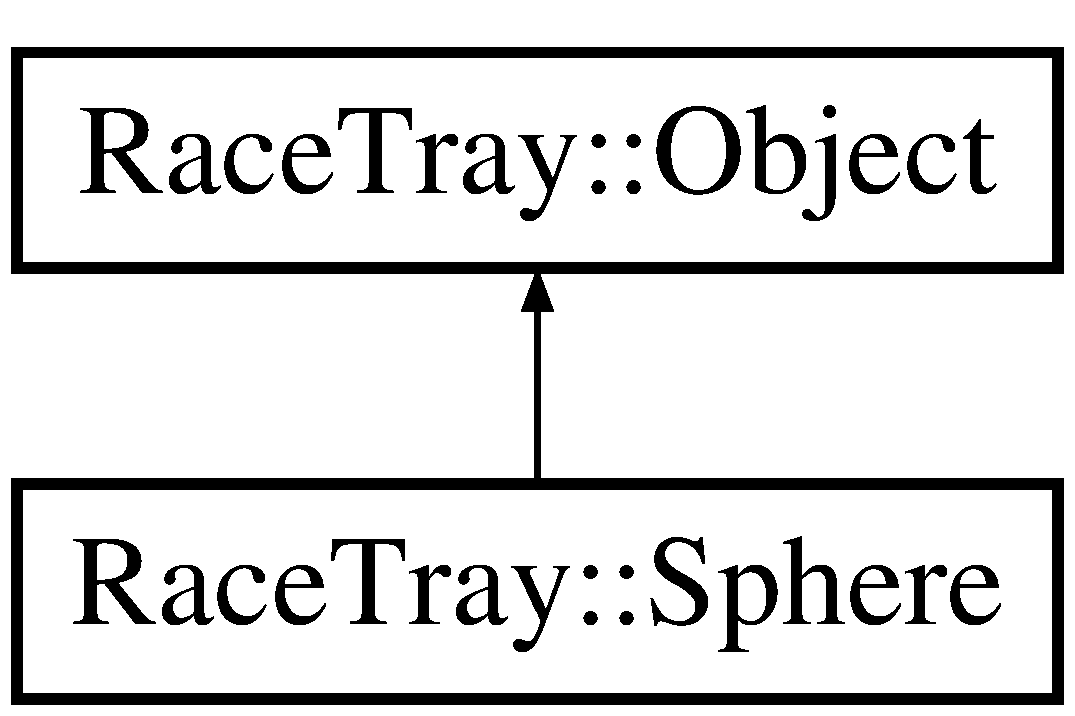
\includegraphics[height=2.000000cm]{class_race_tray_1_1_object}
\end{center}
\end{figure}
\subsection*{Public Member Functions}
\begin{DoxyCompactItemize}
\item 
\hyperlink{class_race_tray_1_1_object_a3d14b748925951286cdc9f7b7d89f7fc}{Object} ()
\item 
\hyperlink{class_race_tray_1_1_object_a71b2eda3dc35db9c3719d8e5d203cb8e}{Object} (const \hyperlink{group___math_gadb6fa781064c3c3c9b13eb984adae162}{Vector3f} \&position)
\item 
\hyperlink{class_race_tray_1_1_object_ad9dd5ecc6017aa2f2054c145ff7830b1}{Object} (const \hyperlink{class_race_tray_1_1_object}{Object} \&other)
\item 
virtual \hyperlink{class_race_tray_1_1_object_aa1d05ba307a8bbeb1c8e01427d6daa58}{$\sim$\-Object} ()
\item 
const \hyperlink{group___math_gadb6fa781064c3c3c9b13eb984adae162}{Vector3f} \& \hyperlink{class_race_tray_1_1_object_a0b5489af58a3195079940162ed7307fe}{get\-Position} () const 
\item 
void \hyperlink{class_race_tray_1_1_object_a2401b3f2bcaaf2fc9f55b3b677d30b77}{set\-Position} (const \hyperlink{group___math_gadb6fa781064c3c3c9b13eb984adae162}{Vector3f} \&value)
\item 
void \hyperlink{class_race_tray_1_1_object_af5b702a62a9d6fd27f0c012df0f2e795}{set\-Material} (const \hyperlink{class_race_tray_1_1_material}{Material} \&material)
\item 
virtual void \hyperlink{class_race_tray_1_1_object_a6ea71904be1d47e93378e58848b6eb87}{check\-Ray\-Collision} (const \hyperlink{group___math_ga5fdea6c2a8db84c0cc5b7aaeeb48b17a}{Rayf} \&ray, \hyperlink{class_race_tray_1_1_scene_collision_data}{Scene\-Collision\-Data} \&data)=0
\end{DoxyCompactItemize}
\subsection*{Protected Attributes}
\begin{DoxyCompactItemize}
\item 
\hyperlink{group___math_gadb6fa781064c3c3c9b13eb984adae162}{Vector3f} \hyperlink{class_race_tray_1_1_object_afc27cf33104f6af734684534e3230723}{\-\_\-position}
\item 
\hyperlink{class_race_tray_1_1_material}{Material} \hyperlink{class_race_tray_1_1_object_a659c1956bd811a2cc687fd899f3aa0e0}{\-\_\-material}
\end{DoxyCompactItemize}


\subsection{Detailed Description}
The base object. All engine entities derive from the base object. 

\subsection{Constructor \& Destructor Documentation}
\hypertarget{class_race_tray_1_1_object_a3d14b748925951286cdc9f7b7d89f7fc}{\index{Race\-Tray\-::\-Object@{Race\-Tray\-::\-Object}!Object@{Object}}
\index{Object@{Object}!RaceTray::Object@{Race\-Tray\-::\-Object}}
\subsubsection[{Object}]{\setlength{\rightskip}{0pt plus 5cm}Race\-Tray\-::\-Object\-::\-Object (
\begin{DoxyParamCaption}
{}
\end{DoxyParamCaption}
)}}\label{class_race_tray_1_1_object_a3d14b748925951286cdc9f7b7d89f7fc}
Default constructor \hypertarget{class_race_tray_1_1_object_a71b2eda3dc35db9c3719d8e5d203cb8e}{\index{Race\-Tray\-::\-Object@{Race\-Tray\-::\-Object}!Object@{Object}}
\index{Object@{Object}!RaceTray::Object@{Race\-Tray\-::\-Object}}
\subsubsection[{Object}]{\setlength{\rightskip}{0pt plus 5cm}Race\-Tray\-::\-Object\-::\-Object (
\begin{DoxyParamCaption}
\item[{const {\bf Vector3f} \&}]{position}
\end{DoxyParamCaption}
)}}\label{class_race_tray_1_1_object_a71b2eda3dc35db9c3719d8e5d203cb8e}
Constructor 
\begin{DoxyParams}{Parameters}
{\em const} & Vector3f The position of the object \\
\hline
\end{DoxyParams}
\hypertarget{class_race_tray_1_1_object_ad9dd5ecc6017aa2f2054c145ff7830b1}{\index{Race\-Tray\-::\-Object@{Race\-Tray\-::\-Object}!Object@{Object}}
\index{Object@{Object}!RaceTray::Object@{Race\-Tray\-::\-Object}}
\subsubsection[{Object}]{\setlength{\rightskip}{0pt plus 5cm}Race\-Tray\-::\-Object\-::\-Object (
\begin{DoxyParamCaption}
\item[{const {\bf Object} \&}]{other}
\end{DoxyParamCaption}
)}}\label{class_race_tray_1_1_object_ad9dd5ecc6017aa2f2054c145ff7830b1}
Copy constructor 
\begin{DoxyParams}{Parameters}
{\em const} & \hyperlink{class_race_tray_1_1_object}{Object}\& The object to copy \\
\hline
\end{DoxyParams}
\hypertarget{class_race_tray_1_1_object_aa1d05ba307a8bbeb1c8e01427d6daa58}{\index{Race\-Tray\-::\-Object@{Race\-Tray\-::\-Object}!$\sim$\-Object@{$\sim$\-Object}}
\index{$\sim$\-Object@{$\sim$\-Object}!RaceTray::Object@{Race\-Tray\-::\-Object}}
\subsubsection[{$\sim$\-Object}]{\setlength{\rightskip}{0pt plus 5cm}Race\-Tray\-::\-Object\-::$\sim$\-Object (
\begin{DoxyParamCaption}
{}
\end{DoxyParamCaption}
)\hspace{0.3cm}{\ttfamily [virtual]}}}\label{class_race_tray_1_1_object_aa1d05ba307a8bbeb1c8e01427d6daa58}
Destructor 

\subsection{Member Function Documentation}
\hypertarget{class_race_tray_1_1_object_a6ea71904be1d47e93378e58848b6eb87}{\index{Race\-Tray\-::\-Object@{Race\-Tray\-::\-Object}!check\-Ray\-Collision@{check\-Ray\-Collision}}
\index{check\-Ray\-Collision@{check\-Ray\-Collision}!RaceTray::Object@{Race\-Tray\-::\-Object}}
\subsubsection[{check\-Ray\-Collision}]{\setlength{\rightskip}{0pt plus 5cm}virtual void Race\-Tray\-::\-Object\-::check\-Ray\-Collision (
\begin{DoxyParamCaption}
\item[{const {\bf Rayf} \&}]{ray, }
\item[{{\bf Scene\-Collision\-Data} \&}]{data}
\end{DoxyParamCaption}
)\hspace{0.3cm}{\ttfamily [pure virtual]}}}\label{class_race_tray_1_1_object_a6ea71904be1d47e93378e58848b6eb87}
Check against this object for a ray collision. 
\begin{DoxyParams}{Parameters}
{\em const} & \hyperlink{class_race_tray_1_1_ray}{Ray}\& The ray against which to check \\
\hline
{\em Scene\-Collision\-Data\&} & The information about the collision, if any \\
\hline
\end{DoxyParams}


Implemented in \hyperlink{class_race_tray_1_1_sphere_a88cf632d6caf1ec6a0ce46efafd6f052}{Race\-Tray\-::\-Sphere}.

\hypertarget{class_race_tray_1_1_object_a0b5489af58a3195079940162ed7307fe}{\index{Race\-Tray\-::\-Object@{Race\-Tray\-::\-Object}!get\-Position@{get\-Position}}
\index{get\-Position@{get\-Position}!RaceTray::Object@{Race\-Tray\-::\-Object}}
\subsubsection[{get\-Position}]{\setlength{\rightskip}{0pt plus 5cm}const {\bf Vector3f} \& Race\-Tray\-::\-Object\-::get\-Position (
\begin{DoxyParamCaption}
{}
\end{DoxyParamCaption}
) const}}\label{class_race_tray_1_1_object_a0b5489af58a3195079940162ed7307fe}
Return the object position \begin{DoxyReturn}{Returns}
const Vector3f\& The object position 
\end{DoxyReturn}
\hypertarget{class_race_tray_1_1_object_af5b702a62a9d6fd27f0c012df0f2e795}{\index{Race\-Tray\-::\-Object@{Race\-Tray\-::\-Object}!set\-Material@{set\-Material}}
\index{set\-Material@{set\-Material}!RaceTray::Object@{Race\-Tray\-::\-Object}}
\subsubsection[{set\-Material}]{\setlength{\rightskip}{0pt plus 5cm}void Race\-Tray\-::\-Object\-::set\-Material (
\begin{DoxyParamCaption}
\item[{const {\bf Material} \&}]{material}
\end{DoxyParamCaption}
)}}\label{class_race_tray_1_1_object_af5b702a62a9d6fd27f0c012df0f2e795}
Set the material for the object 
\begin{DoxyParams}{Parameters}
{\em const} & \hyperlink{class_race_tray_1_1_material}{Material}\& The material to set for this object \\
\hline
\end{DoxyParams}
\hypertarget{class_race_tray_1_1_object_a2401b3f2bcaaf2fc9f55b3b677d30b77}{\index{Race\-Tray\-::\-Object@{Race\-Tray\-::\-Object}!set\-Position@{set\-Position}}
\index{set\-Position@{set\-Position}!RaceTray::Object@{Race\-Tray\-::\-Object}}
\subsubsection[{set\-Position}]{\setlength{\rightskip}{0pt plus 5cm}void Race\-Tray\-::\-Object\-::set\-Position (
\begin{DoxyParamCaption}
\item[{const {\bf Vector3f} \&}]{value}
\end{DoxyParamCaption}
)}}\label{class_race_tray_1_1_object_a2401b3f2bcaaf2fc9f55b3b677d30b77}
Set the object position 
\begin{DoxyParams}{Parameters}
{\em const} & Vector3f\& The new position \\
\hline
\end{DoxyParams}


\subsection{Member Data Documentation}
\hypertarget{class_race_tray_1_1_object_a659c1956bd811a2cc687fd899f3aa0e0}{\index{Race\-Tray\-::\-Object@{Race\-Tray\-::\-Object}!\-\_\-material@{\-\_\-material}}
\index{\-\_\-material@{\-\_\-material}!RaceTray::Object@{Race\-Tray\-::\-Object}}
\subsubsection[{\-\_\-material}]{\setlength{\rightskip}{0pt plus 5cm}{\bf Material} Race\-Tray\-::\-Object\-::\-\_\-material\hspace{0.3cm}{\ttfamily [protected]}}}\label{class_race_tray_1_1_object_a659c1956bd811a2cc687fd899f3aa0e0}
The object's material \hypertarget{class_race_tray_1_1_object_afc27cf33104f6af734684534e3230723}{\index{Race\-Tray\-::\-Object@{Race\-Tray\-::\-Object}!\-\_\-position@{\-\_\-position}}
\index{\-\_\-position@{\-\_\-position}!RaceTray::Object@{Race\-Tray\-::\-Object}}
\subsubsection[{\-\_\-position}]{\setlength{\rightskip}{0pt plus 5cm}{\bf Vector3f} Race\-Tray\-::\-Object\-::\-\_\-position\hspace{0.3cm}{\ttfamily [protected]}}}\label{class_race_tray_1_1_object_afc27cf33104f6af734684534e3230723}
Position of the object 

The documentation for this class was generated from the following files\-:\begin{DoxyCompactItemize}
\item 
C\-:/\-Users/\-Gael/\-Documents/\-Race\-Tray/\-Geometry/R\-T\-Object.\-h\item 
C\-:/\-Users/\-Gael/\-Documents/\-Race\-Tray/\-Geometry/R\-T\-Object.\-cpp\end{DoxyCompactItemize}

\hypertarget{class_race_tray_1_1_ray}{\section{Race\-Tray\-:\-:Ray$<$ Unit $>$ Class Template Reference}
\label{class_race_tray_1_1_ray}\index{Race\-Tray\-::\-Ray$<$ Unit $>$@{Race\-Tray\-::\-Ray$<$ Unit $>$}}
}


{\ttfamily \#include $<$R\-T\-Ray.\-h$>$}

\subsection*{Public Member Functions}
\begin{DoxyCompactItemize}
\item 
\hyperlink{group___math_ga2e3d2c29f2df4ab3da10da79d4acb852}{Ray} ()
\item 
\hyperlink{group___math_gabe89aef5906b96af94ad94ad0deba455}{Ray} (const \hyperlink{class_race_tray_1_1_vector3}{Vector3}$<$ Unit $>$ \&origin, const \hyperlink{class_race_tray_1_1_vector3}{Vector3}$<$ Unit $>$ \&direction)
\item 
\hyperlink{group___math_ga8e46b1356e03d968ffd813076d6818b2}{Ray} (const \hyperlink{class_race_tray_1_1_ray}{Ray} \&other)
\item 
\hyperlink{group___math_ga8b0e575ce5df046c0c7615c32a96a46f}{$\sim$\-Ray} ()
\item 
const \hyperlink{class_race_tray_1_1_vector3}{Vector3}$<$ Unit $>$ \& \hyperlink{group___math_gab1690c909fff67ff5c878aa6f05bfe2b}{get\-Origin} () const 
\item 
const \hyperlink{class_race_tray_1_1_vector3}{Vector3}$<$ Unit $>$ \& \hyperlink{group___math_gaab0b0ed57af0899286c2996dfdc9418b}{get\-Direction} () const 
\end{DoxyCompactItemize}


\subsection{Detailed Description}
\subsubsection*{template$<$typename Unit$>$class Race\-Tray\-::\-Ray$<$ Unit $>$}

Represents a ray in 3 dimensional space defined as an origin vector and a direction vector 

The documentation for this class was generated from the following files\-:\begin{DoxyCompactItemize}
\item 
C\-:/\-Users/\-Gael/\-Documents/\-Race\-Tray/\-Math/R\-T\-Math\-Prerequisites.\-h\item 
C\-:/\-Users/\-Gael/\-Documents/\-Race\-Tray/\-Math/R\-T\-Ray.\-h\item 
C\-:/\-Users/\-Gael/\-Documents/\-Race\-Tray/\-Math/R\-T\-Ray.\-inl\end{DoxyCompactItemize}

\hypertarget{class_race_tray_1_1_renderer}{\section{Race\-Tray\-:\-:Renderer Class Reference}
\label{class_race_tray_1_1_renderer}\index{Race\-Tray\-::\-Renderer@{Race\-Tray\-::\-Renderer}}
}


{\ttfamily \#include $<$R\-T\-Renderer.\-h$>$}

\subsection*{Public Member Functions}
\begin{DoxyCompactItemize}
\item 
\hyperlink{class_race_tray_1_1_renderer_a83cc3c485a1ccaab2148f93698e52398}{Renderer} ()
\item 
\hyperlink{class_race_tray_1_1_renderer_a4569bede271aef7ed70e0b99018ef721}{$\sim$\-Renderer} ()
\item 
bool \hyperlink{class_race_tray_1_1_renderer_ac74c0a08970ff3c28a6c0c333ceeb7e2}{initialize} ()
\item 
void \hyperlink{class_race_tray_1_1_renderer_ae69c470e128ab281c1ce947ba9f2a77f}{destroy} ()
\item 
bool \hyperlink{class_race_tray_1_1_renderer_a8538367f6ab111b44089376de2dfeadb}{render} (const \hyperlink{class_race_tray_1_1_scene_graph}{Scene\-Graph} $\ast$scene\-Graph, const std\-::vector$<$ \hyperlink{class_race_tray_1_1_light}{Light} $\ast$ $>$ \&lights, const \hyperlink{class_race_tray_1_1_camera}{Camera} \&camera)
\end{DoxyCompactItemize}


\subsection{Detailed Description}
\hyperlink{class_race_tray_1_1_renderer}{Renderer} owns the rendering pipeline. It is responsible for applying colors to the frame and flushing the output when done. 

\subsection{Constructor \& Destructor Documentation}
\hypertarget{class_race_tray_1_1_renderer_a83cc3c485a1ccaab2148f93698e52398}{\index{Race\-Tray\-::\-Renderer@{Race\-Tray\-::\-Renderer}!Renderer@{Renderer}}
\index{Renderer@{Renderer}!RaceTray::Renderer@{Race\-Tray\-::\-Renderer}}
\subsubsection[{Renderer}]{\setlength{\rightskip}{0pt plus 5cm}Race\-Tray\-::\-Renderer\-::\-Renderer (
\begin{DoxyParamCaption}
{}
\end{DoxyParamCaption}
)}}\label{class_race_tray_1_1_renderer_a83cc3c485a1ccaab2148f93698e52398}
Default constructor \hypertarget{class_race_tray_1_1_renderer_a4569bede271aef7ed70e0b99018ef721}{\index{Race\-Tray\-::\-Renderer@{Race\-Tray\-::\-Renderer}!$\sim$\-Renderer@{$\sim$\-Renderer}}
\index{$\sim$\-Renderer@{$\sim$\-Renderer}!RaceTray::Renderer@{Race\-Tray\-::\-Renderer}}
\subsubsection[{$\sim$\-Renderer}]{\setlength{\rightskip}{0pt plus 5cm}Race\-Tray\-::\-Renderer\-::$\sim$\-Renderer (
\begin{DoxyParamCaption}
{}
\end{DoxyParamCaption}
)}}\label{class_race_tray_1_1_renderer_a4569bede271aef7ed70e0b99018ef721}
Destructor 

\subsection{Member Function Documentation}
\hypertarget{class_race_tray_1_1_renderer_ae69c470e128ab281c1ce947ba9f2a77f}{\index{Race\-Tray\-::\-Renderer@{Race\-Tray\-::\-Renderer}!destroy@{destroy}}
\index{destroy@{destroy}!RaceTray::Renderer@{Race\-Tray\-::\-Renderer}}
\subsubsection[{destroy}]{\setlength{\rightskip}{0pt plus 5cm}void Race\-Tray\-::\-Renderer\-::destroy (
\begin{DoxyParamCaption}
{}
\end{DoxyParamCaption}
)}}\label{class_race_tray_1_1_renderer_ae69c470e128ab281c1ce947ba9f2a77f}
Destroy the renderer and all its components \hypertarget{class_race_tray_1_1_renderer_ac74c0a08970ff3c28a6c0c333ceeb7e2}{\index{Race\-Tray\-::\-Renderer@{Race\-Tray\-::\-Renderer}!initialize@{initialize}}
\index{initialize@{initialize}!RaceTray::Renderer@{Race\-Tray\-::\-Renderer}}
\subsubsection[{initialize}]{\setlength{\rightskip}{0pt plus 5cm}bool Race\-Tray\-::\-Renderer\-::initialize (
\begin{DoxyParamCaption}
{}
\end{DoxyParamCaption}
)}}\label{class_race_tray_1_1_renderer_ac74c0a08970ff3c28a6c0c333ceeb7e2}
Initialize the renderer, including the output buffer \begin{DoxyReturn}{Returns}
bool Return true if the initialization succeeded 
\end{DoxyReturn}
\hypertarget{class_race_tray_1_1_renderer_a8538367f6ab111b44089376de2dfeadb}{\index{Race\-Tray\-::\-Renderer@{Race\-Tray\-::\-Renderer}!render@{render}}
\index{render@{render}!RaceTray::Renderer@{Race\-Tray\-::\-Renderer}}
\subsubsection[{render}]{\setlength{\rightskip}{0pt plus 5cm}bool Race\-Tray\-::\-Renderer\-::render (
\begin{DoxyParamCaption}
\item[{const {\bf Scene\-Graph} $\ast$}]{scene\-Graph, }
\item[{const std\-::vector$<$ {\bf Light} $\ast$ $>$ \&}]{lights, }
\item[{const {\bf Camera} \&}]{camera}
\end{DoxyParamCaption}
)}}\label{class_race_tray_1_1_renderer_a8538367f6ab111b44089376de2dfeadb}
Given the scene graph, camera, and lights, render the scene to the target output 
\begin{DoxyParams}{Parameters}
{\em const} & Scene\-Graph$\ast$ The \hyperlink{class_race_tray_1_1_scene_graph}{Scene\-Graph} instance against which to render \\
\hline
{\em const} & vector$<$\-Light$\ast$$>$\& The vector holding all the light data in the scene \\
\hline
{\em const} & \hyperlink{class_race_tray_1_1_camera}{Camera}\& The scene's camera \\
\hline
\end{DoxyParams}


The documentation for this class was generated from the following files\-:\begin{DoxyCompactItemize}
\item 
C\-:/\-Users/\-Gael/\-Documents/\-Race\-Tray/\-Scene/R\-T\-Renderer.\-h\item 
C\-:/\-Users/\-Gael/\-Documents/\-Race\-Tray/\-Scene/R\-T\-Renderer.\-cpp\end{DoxyCompactItemize}

\hypertarget{class_race_tray_1_1_render_target}{\section{Race\-Tray\-:\-:Render\-Target Class Reference}
\label{class_race_tray_1_1_render_target}\index{Race\-Tray\-::\-Render\-Target@{Race\-Tray\-::\-Render\-Target}}
}


{\ttfamily \#include $<$R\-T\-Render\-Target.\-h$>$}

Inheritance diagram for Race\-Tray\-:\-:Render\-Target\-:\begin{figure}[H]
\begin{center}
\leavevmode
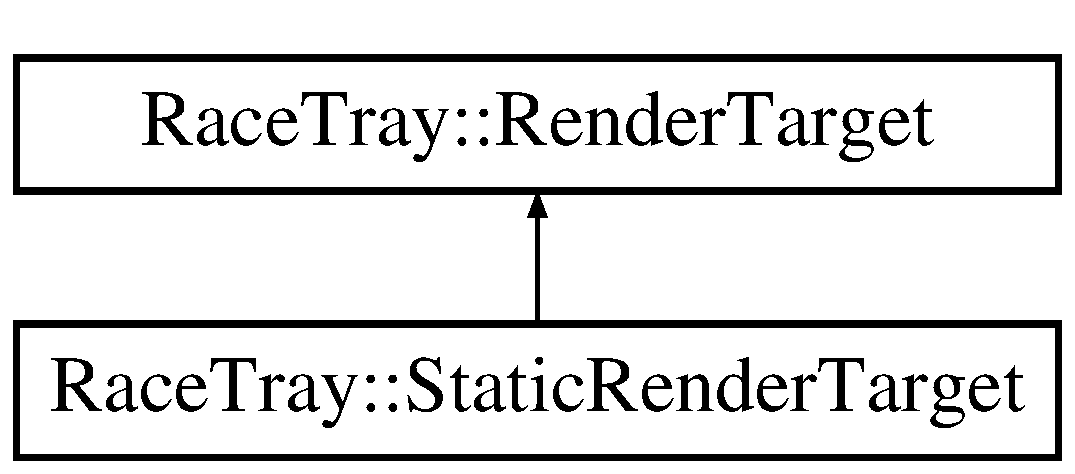
\includegraphics[height=2.000000cm]{class_race_tray_1_1_render_target}
\end{center}
\end{figure}
\subsection*{Public Member Functions}
\begin{DoxyCompactItemize}
\item 
\hyperlink{class_race_tray_1_1_render_target_a19af1e6e8c1d05d95f8a3d6443540d85}{Render\-Target} ()
\item 
virtual \hyperlink{class_race_tray_1_1_render_target_a18c35ced54cd155cd654efbac788e3a1}{$\sim$\-Render\-Target} ()
\item 
virtual bool \hyperlink{class_race_tray_1_1_render_target_a8ac06cc0f9af87e3373cd1514f64b76c}{initialize} (int width, int height)=0
\item 
virtual void \hyperlink{class_race_tray_1_1_render_target_a9e4e394b421102e5edaea14411dc28bd}{destroy} ()=0
\end{DoxyCompactItemize}
\subsection*{Protected Attributes}
\begin{DoxyCompactItemize}
\item 
int \hyperlink{class_race_tray_1_1_render_target_a26912f27dd5d06467d2144049610057d}{\-\_\-width}
\item 
int \hyperlink{class_race_tray_1_1_render_target_af3c0dcb0091c5c5be2b3350fa8dce79b}{\-\_\-height}
\end{DoxyCompactItemize}


\subsection{Detailed Description}
The render target is the target output during the scene render process. Each pixels gets copied to the target before the final draw call is made. 

\subsection{Constructor \& Destructor Documentation}
\hypertarget{class_race_tray_1_1_render_target_a19af1e6e8c1d05d95f8a3d6443540d85}{\index{Race\-Tray\-::\-Render\-Target@{Race\-Tray\-::\-Render\-Target}!Render\-Target@{Render\-Target}}
\index{Render\-Target@{Render\-Target}!RaceTray::RenderTarget@{Race\-Tray\-::\-Render\-Target}}
\subsubsection[{Render\-Target}]{\setlength{\rightskip}{0pt plus 5cm}Race\-Tray\-::\-Render\-Target\-::\-Render\-Target (
\begin{DoxyParamCaption}
{}
\end{DoxyParamCaption}
)}}\label{class_race_tray_1_1_render_target_a19af1e6e8c1d05d95f8a3d6443540d85}
Default constructor \hypertarget{class_race_tray_1_1_render_target_a18c35ced54cd155cd654efbac788e3a1}{\index{Race\-Tray\-::\-Render\-Target@{Race\-Tray\-::\-Render\-Target}!$\sim$\-Render\-Target@{$\sim$\-Render\-Target}}
\index{$\sim$\-Render\-Target@{$\sim$\-Render\-Target}!RaceTray::RenderTarget@{Race\-Tray\-::\-Render\-Target}}
\subsubsection[{$\sim$\-Render\-Target}]{\setlength{\rightskip}{0pt plus 5cm}Race\-Tray\-::\-Render\-Target\-::$\sim$\-Render\-Target (
\begin{DoxyParamCaption}
{}
\end{DoxyParamCaption}
)\hspace{0.3cm}{\ttfamily [virtual]}}}\label{class_race_tray_1_1_render_target_a18c35ced54cd155cd654efbac788e3a1}
Destructor 

\subsection{Member Function Documentation}
\hypertarget{class_race_tray_1_1_render_target_a9e4e394b421102e5edaea14411dc28bd}{\index{Race\-Tray\-::\-Render\-Target@{Race\-Tray\-::\-Render\-Target}!destroy@{destroy}}
\index{destroy@{destroy}!RaceTray::RenderTarget@{Race\-Tray\-::\-Render\-Target}}
\subsubsection[{destroy}]{\setlength{\rightskip}{0pt plus 5cm}virtual void Race\-Tray\-::\-Render\-Target\-::destroy (
\begin{DoxyParamCaption}
{}
\end{DoxyParamCaption}
)\hspace{0.3cm}{\ttfamily [pure virtual]}}}\label{class_race_tray_1_1_render_target_a9e4e394b421102e5edaea14411dc28bd}
Destroy the render target 

Implemented in \hyperlink{class_race_tray_1_1_static_render_target_a4f163966507ea68a0eccf7c3f5959bd3}{Race\-Tray\-::\-Static\-Render\-Target}.

\hypertarget{class_race_tray_1_1_render_target_a8ac06cc0f9af87e3373cd1514f64b76c}{\index{Race\-Tray\-::\-Render\-Target@{Race\-Tray\-::\-Render\-Target}!initialize@{initialize}}
\index{initialize@{initialize}!RaceTray::RenderTarget@{Race\-Tray\-::\-Render\-Target}}
\subsubsection[{initialize}]{\setlength{\rightskip}{0pt plus 5cm}virtual bool Race\-Tray\-::\-Render\-Target\-::initialize (
\begin{DoxyParamCaption}
\item[{int}]{width, }
\item[{int}]{height}
\end{DoxyParamCaption}
)\hspace{0.3cm}{\ttfamily [pure virtual]}}}\label{class_race_tray_1_1_render_target_a8ac06cc0f9af87e3373cd1514f64b76c}
Initialize the render target 
\begin{DoxyParams}{Parameters}
{\em int} & The width of the render target \\
\hline
{\em height} & The height of the render target \\
\hline
\end{DoxyParams}
\begin{DoxyReturn}{Returns}
bool Returns true if the target is successfully created 
\end{DoxyReturn}


Implemented in \hyperlink{class_race_tray_1_1_static_render_target_a4f7bf1080af87d6b64e40771adac1861}{Race\-Tray\-::\-Static\-Render\-Target}.



\subsection{Member Data Documentation}
\hypertarget{class_race_tray_1_1_render_target_af3c0dcb0091c5c5be2b3350fa8dce79b}{\index{Race\-Tray\-::\-Render\-Target@{Race\-Tray\-::\-Render\-Target}!\-\_\-height@{\-\_\-height}}
\index{\-\_\-height@{\-\_\-height}!RaceTray::RenderTarget@{Race\-Tray\-::\-Render\-Target}}
\subsubsection[{\-\_\-height}]{\setlength{\rightskip}{0pt plus 5cm}int Race\-Tray\-::\-Render\-Target\-::\-\_\-height\hspace{0.3cm}{\ttfamily [protected]}}}\label{class_race_tray_1_1_render_target_af3c0dcb0091c5c5be2b3350fa8dce79b}
The height of the render target \hypertarget{class_race_tray_1_1_render_target_a26912f27dd5d06467d2144049610057d}{\index{Race\-Tray\-::\-Render\-Target@{Race\-Tray\-::\-Render\-Target}!\-\_\-width@{\-\_\-width}}
\index{\-\_\-width@{\-\_\-width}!RaceTray::RenderTarget@{Race\-Tray\-::\-Render\-Target}}
\subsubsection[{\-\_\-width}]{\setlength{\rightskip}{0pt plus 5cm}int Race\-Tray\-::\-Render\-Target\-::\-\_\-width\hspace{0.3cm}{\ttfamily [protected]}}}\label{class_race_tray_1_1_render_target_a26912f27dd5d06467d2144049610057d}
The width of the render target 

The documentation for this class was generated from the following files\-:\begin{DoxyCompactItemize}
\item 
C\-:/\-Users/\-Gael/\-Documents/\-Race\-Tray/\-Scene/R\-T\-Render\-Target.\-h\item 
C\-:/\-Users/\-Gael/\-Documents/\-Race\-Tray/\-Scene/R\-T\-Render\-Target.\-cpp\end{DoxyCompactItemize}

\hypertarget{class_race_tray_1_1_scene}{\section{Race\-Tray\-:\-:Scene Class Reference}
\label{class_race_tray_1_1_scene}\index{Race\-Tray\-::\-Scene@{Race\-Tray\-::\-Scene}}
}


{\ttfamily \#include $<$R\-T\-Scene.\-h$>$}

\subsection*{Public Member Functions}
\begin{DoxyCompactItemize}
\item 
\hyperlink{class_race_tray_1_1_scene_ab0b893217e6108982c963586a3eed7a1}{Scene} ()
\item 
\hyperlink{class_race_tray_1_1_scene_a64dbc6679f6543c06229efc87725532b}{Scene} (const \hyperlink{class_race_tray_1_1_scene}{Scene} \&other)
\item 
\hyperlink{class_race_tray_1_1_scene_af7c0fb4d0f3d4a10b50fb340376eed21}{$\sim$\-Scene} ()
\item 
bool \hyperlink{class_race_tray_1_1_scene_a6c01bc164fe3188f9de317b5176bcd18}{initialize} ()
\item 
void \hyperlink{class_race_tray_1_1_scene_abf3e9e56a8d5af553d0805fbdc807aeb}{destroy} ()
\item 
bool \hyperlink{class_race_tray_1_1_scene_a50293de9c949fbf279549d6618aa7dfb}{play} ()
\item 
void \hyperlink{class_race_tray_1_1_scene_aee10122e6078860b355900ff978832b1}{register\-Camera} (\hyperlink{class_race_tray_1_1_camera}{Camera} $\ast$camera)
\item 
void \hyperlink{class_race_tray_1_1_scene_a5501e7115475096e3b5753a209cf4af0}{add\-Renderable} (\hyperlink{class_race_tray_1_1_object}{Object} $\ast$object)
\end{DoxyCompactItemize}


\subsection{Detailed Description}
A scene is the overarching container for all data within the Race\-Tray ray tracer. The scene the scene graph, physics world, animation sequences, the render pipeline, and the application configuration. 

\subsection{Constructor \& Destructor Documentation}
\hypertarget{class_race_tray_1_1_scene_ab0b893217e6108982c963586a3eed7a1}{\index{Race\-Tray\-::\-Scene@{Race\-Tray\-::\-Scene}!Scene@{Scene}}
\index{Scene@{Scene}!RaceTray::Scene@{Race\-Tray\-::\-Scene}}
\subsubsection[{Scene}]{\setlength{\rightskip}{0pt plus 5cm}Race\-Tray\-::\-Scene\-::\-Scene (
\begin{DoxyParamCaption}
{}
\end{DoxyParamCaption}
)}}\label{class_race_tray_1_1_scene_ab0b893217e6108982c963586a3eed7a1}
Default constructor \hypertarget{class_race_tray_1_1_scene_a64dbc6679f6543c06229efc87725532b}{\index{Race\-Tray\-::\-Scene@{Race\-Tray\-::\-Scene}!Scene@{Scene}}
\index{Scene@{Scene}!RaceTray::Scene@{Race\-Tray\-::\-Scene}}
\subsubsection[{Scene}]{\setlength{\rightskip}{0pt plus 5cm}Race\-Tray\-::\-Scene\-::\-Scene (
\begin{DoxyParamCaption}
\item[{const {\bf Scene} \&}]{other}
\end{DoxyParamCaption}
)}}\label{class_race_tray_1_1_scene_a64dbc6679f6543c06229efc87725532b}
Copy constructor 
\begin{DoxyParams}{Parameters}
{\em const} & \hyperlink{class_race_tray_1_1_scene}{Scene}\& The scene to copy \\
\hline
\end{DoxyParams}
\hypertarget{class_race_tray_1_1_scene_af7c0fb4d0f3d4a10b50fb340376eed21}{\index{Race\-Tray\-::\-Scene@{Race\-Tray\-::\-Scene}!$\sim$\-Scene@{$\sim$\-Scene}}
\index{$\sim$\-Scene@{$\sim$\-Scene}!RaceTray::Scene@{Race\-Tray\-::\-Scene}}
\subsubsection[{$\sim$\-Scene}]{\setlength{\rightskip}{0pt plus 5cm}Race\-Tray\-::\-Scene\-::$\sim$\-Scene (
\begin{DoxyParamCaption}
{}
\end{DoxyParamCaption}
)}}\label{class_race_tray_1_1_scene_af7c0fb4d0f3d4a10b50fb340376eed21}
Destructor 

\subsection{Member Function Documentation}
\hypertarget{class_race_tray_1_1_scene_a5501e7115475096e3b5753a209cf4af0}{\index{Race\-Tray\-::\-Scene@{Race\-Tray\-::\-Scene}!add\-Renderable@{add\-Renderable}}
\index{add\-Renderable@{add\-Renderable}!RaceTray::Scene@{Race\-Tray\-::\-Scene}}
\subsubsection[{add\-Renderable}]{\setlength{\rightskip}{0pt plus 5cm}void Race\-Tray\-::\-Scene\-::add\-Renderable (
\begin{DoxyParamCaption}
\item[{{\bf Object} $\ast$}]{object}
\end{DoxyParamCaption}
)}}\label{class_race_tray_1_1_scene_a5501e7115475096e3b5753a209cf4af0}
Add a renderable object to the scene 
\begin{DoxyParams}{Parameters}
{\em Object$\ast$} & The object to add to the scene graph \\
\hline
\end{DoxyParams}
\hypertarget{class_race_tray_1_1_scene_abf3e9e56a8d5af553d0805fbdc807aeb}{\index{Race\-Tray\-::\-Scene@{Race\-Tray\-::\-Scene}!destroy@{destroy}}
\index{destroy@{destroy}!RaceTray::Scene@{Race\-Tray\-::\-Scene}}
\subsubsection[{destroy}]{\setlength{\rightskip}{0pt plus 5cm}void Race\-Tray\-::\-Scene\-::destroy (
\begin{DoxyParamCaption}
{}
\end{DoxyParamCaption}
)}}\label{class_race_tray_1_1_scene_abf3e9e56a8d5af553d0805fbdc807aeb}
Destroy the scene and free all resources used. \hypertarget{class_race_tray_1_1_scene_a6c01bc164fe3188f9de317b5176bcd18}{\index{Race\-Tray\-::\-Scene@{Race\-Tray\-::\-Scene}!initialize@{initialize}}
\index{initialize@{initialize}!RaceTray::Scene@{Race\-Tray\-::\-Scene}}
\subsubsection[{initialize}]{\setlength{\rightskip}{0pt plus 5cm}bool Race\-Tray\-::\-Scene\-::initialize (
\begin{DoxyParamCaption}
{}
\end{DoxyParamCaption}
)}}\label{class_race_tray_1_1_scene_a6c01bc164fe3188f9de317b5176bcd18}
Initialize the scene. This takes care of reading in any configuration files specified and preparing the scene to be played. \begin{DoxyReturn}{Returns}
bool Returns true if the scene was initialized successfully 
\end{DoxyReturn}
\hypertarget{class_race_tray_1_1_scene_a50293de9c949fbf279549d6618aa7dfb}{\index{Race\-Tray\-::\-Scene@{Race\-Tray\-::\-Scene}!play@{play}}
\index{play@{play}!RaceTray::Scene@{Race\-Tray\-::\-Scene}}
\subsubsection[{play}]{\setlength{\rightskip}{0pt plus 5cm}bool Race\-Tray\-::\-Scene\-::play (
\begin{DoxyParamCaption}
{}
\end{DoxyParamCaption}
)}}\label{class_race_tray_1_1_scene_a50293de9c949fbf279549d6618aa7dfb}
Play the scene \begin{DoxyReturn}{Returns}
bool Returns true if the scene was played successfully 
\end{DoxyReturn}
\hypertarget{class_race_tray_1_1_scene_aee10122e6078860b355900ff978832b1}{\index{Race\-Tray\-::\-Scene@{Race\-Tray\-::\-Scene}!register\-Camera@{register\-Camera}}
\index{register\-Camera@{register\-Camera}!RaceTray::Scene@{Race\-Tray\-::\-Scene}}
\subsubsection[{register\-Camera}]{\setlength{\rightskip}{0pt plus 5cm}void Race\-Tray\-::\-Scene\-::register\-Camera (
\begin{DoxyParamCaption}
\item[{{\bf Camera} $\ast$}]{camera}
\end{DoxyParamCaption}
)}}\label{class_race_tray_1_1_scene_aee10122e6078860b355900ff978832b1}
Register a camera with the scene and set it as the active camera 
\begin{DoxyParams}{Parameters}
{\em Camera$\ast$} & The camera to register \\
\hline
\end{DoxyParams}


The documentation for this class was generated from the following files\-:\begin{DoxyCompactItemize}
\item 
C\-:/\-Users/\-Gael/\-Documents/\-Race\-Tray/\-Scene/R\-T\-Scene.\-h\item 
C\-:/\-Users/\-Gael/\-Documents/\-Race\-Tray/\-Scene/R\-T\-Scene.\-cpp\end{DoxyCompactItemize}

\hypertarget{class_race_tray_1_1_scene_builder}{\section{Race\-Tray\-:\-:Scene\-Builder Class Reference}
\label{class_race_tray_1_1_scene_builder}\index{Race\-Tray\-::\-Scene\-Builder@{Race\-Tray\-::\-Scene\-Builder}}
}


{\ttfamily \#include $<$R\-T\-Scene\-Builder.\-h$>$}

Inheritance diagram for Race\-Tray\-:\-:Scene\-Builder\-:\begin{figure}[H]
\begin{center}
\leavevmode
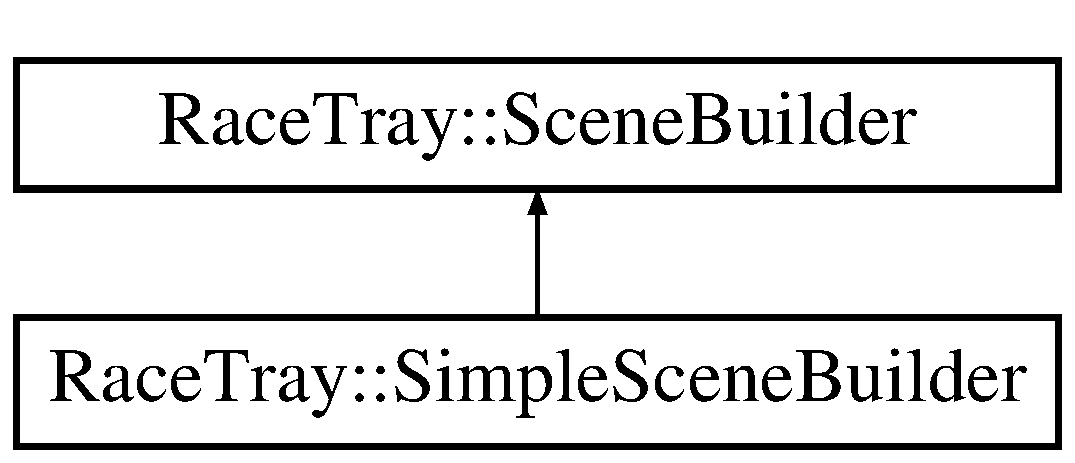
\includegraphics[height=2.000000cm]{class_race_tray_1_1_scene_builder}
\end{center}
\end{figure}
\subsection*{Public Member Functions}
\begin{DoxyCompactItemize}
\item 
\hyperlink{class_race_tray_1_1_scene_builder_a0669208713bfb4355d5a4769790c97a4}{Scene\-Builder} ()
\item 
virtual \hyperlink{class_race_tray_1_1_scene_builder_a6c1b61bbe691660c4d5dfdb8ce7a0949}{$\sim$\-Scene\-Builder} ()
\item 
virtual bool \hyperlink{class_race_tray_1_1_scene_builder_abc2dfdc80fe63a47292e5d6f4618d26f}{build\-Scene} (\hyperlink{class_race_tray_1_1_scene}{Scene} $\ast$scene)=0
\end{DoxyCompactItemize}


\subsection{Detailed Description}
Base class that is responsible for constructing a scene. 

\subsection{Constructor \& Destructor Documentation}
\hypertarget{class_race_tray_1_1_scene_builder_a0669208713bfb4355d5a4769790c97a4}{\index{Race\-Tray\-::\-Scene\-Builder@{Race\-Tray\-::\-Scene\-Builder}!Scene\-Builder@{Scene\-Builder}}
\index{Scene\-Builder@{Scene\-Builder}!RaceTray::SceneBuilder@{Race\-Tray\-::\-Scene\-Builder}}
\subsubsection[{Scene\-Builder}]{\setlength{\rightskip}{0pt plus 5cm}Race\-Tray\-::\-Scene\-Builder\-::\-Scene\-Builder (
\begin{DoxyParamCaption}
{}
\end{DoxyParamCaption}
)}}\label{class_race_tray_1_1_scene_builder_a0669208713bfb4355d5a4769790c97a4}
Default constructor \hypertarget{class_race_tray_1_1_scene_builder_a6c1b61bbe691660c4d5dfdb8ce7a0949}{\index{Race\-Tray\-::\-Scene\-Builder@{Race\-Tray\-::\-Scene\-Builder}!$\sim$\-Scene\-Builder@{$\sim$\-Scene\-Builder}}
\index{$\sim$\-Scene\-Builder@{$\sim$\-Scene\-Builder}!RaceTray::SceneBuilder@{Race\-Tray\-::\-Scene\-Builder}}
\subsubsection[{$\sim$\-Scene\-Builder}]{\setlength{\rightskip}{0pt plus 5cm}Race\-Tray\-::\-Scene\-Builder\-::$\sim$\-Scene\-Builder (
\begin{DoxyParamCaption}
{}
\end{DoxyParamCaption}
)\hspace{0.3cm}{\ttfamily [virtual]}}}\label{class_race_tray_1_1_scene_builder_a6c1b61bbe691660c4d5dfdb8ce7a0949}
Destructor 

\subsection{Member Function Documentation}
\hypertarget{class_race_tray_1_1_scene_builder_abc2dfdc80fe63a47292e5d6f4618d26f}{\index{Race\-Tray\-::\-Scene\-Builder@{Race\-Tray\-::\-Scene\-Builder}!build\-Scene@{build\-Scene}}
\index{build\-Scene@{build\-Scene}!RaceTray::SceneBuilder@{Race\-Tray\-::\-Scene\-Builder}}
\subsubsection[{build\-Scene}]{\setlength{\rightskip}{0pt plus 5cm}virtual bool Race\-Tray\-::\-Scene\-Builder\-::build\-Scene (
\begin{DoxyParamCaption}
\item[{{\bf Scene} $\ast$}]{scene}
\end{DoxyParamCaption}
)\hspace{0.3cm}{\ttfamily [pure virtual]}}}\label{class_race_tray_1_1_scene_builder_abc2dfdc80fe63a47292e5d6f4618d26f}
Build the scene 
\begin{DoxyParams}{Parameters}
{\em Scene$\ast$} & The scene to build \\
\hline
\end{DoxyParams}


Implemented in \hyperlink{class_race_tray_1_1_simple_scene_builder_ae4a08c2dae004e17f95a30cbf8249c8b}{Race\-Tray\-::\-Simple\-Scene\-Builder}.



The documentation for this class was generated from the following files\-:\begin{DoxyCompactItemize}
\item 
C\-:/\-Users/\-Gael/\-Documents/\-Race\-Tray/\-Scene/R\-T\-Scene\-Builder.\-h\item 
C\-:/\-Users/\-Gael/\-Documents/\-Race\-Tray/\-Scene/R\-T\-Scene\-Builder.\-cpp\end{DoxyCompactItemize}

\hypertarget{class_race_tray_1_1_scene_collision_data}{\section{Race\-Tray\-:\-:Scene\-Collision\-Data Class Reference}
\label{class_race_tray_1_1_scene_collision_data}\index{Race\-Tray\-::\-Scene\-Collision\-Data@{Race\-Tray\-::\-Scene\-Collision\-Data}}
}


{\ttfamily \#include $<$R\-T\-Scene\-Collision\-Data.\-h$>$}

\subsection*{Public Member Functions}
\begin{DoxyCompactItemize}
\item 
\hyperlink{class_race_tray_1_1_scene_collision_data_aba090f8f91f7bee2a81ac55730d91ced}{Scene\-Collision\-Data} ()
\end{DoxyCompactItemize}


\subsection{Detailed Description}
Contains information about a ray-\/scene collision. Primarily holds the origin ray, the intersecting object, the contact point, and the contact normal. 

\subsection{Constructor \& Destructor Documentation}
\hypertarget{class_race_tray_1_1_scene_collision_data_aba090f8f91f7bee2a81ac55730d91ced}{\index{Race\-Tray\-::\-Scene\-Collision\-Data@{Race\-Tray\-::\-Scene\-Collision\-Data}!Scene\-Collision\-Data@{Scene\-Collision\-Data}}
\index{Scene\-Collision\-Data@{Scene\-Collision\-Data}!RaceTray::SceneCollisionData@{Race\-Tray\-::\-Scene\-Collision\-Data}}
\subsubsection[{Scene\-Collision\-Data}]{\setlength{\rightskip}{0pt plus 5cm}Race\-Tray\-::\-Scene\-Collision\-Data\-::\-Scene\-Collision\-Data (
\begin{DoxyParamCaption}
{}
\end{DoxyParamCaption}
)}}\label{class_race_tray_1_1_scene_collision_data_aba090f8f91f7bee2a81ac55730d91ced}
Default constructor 

The documentation for this class was generated from the following files\-:\begin{DoxyCompactItemize}
\item 
C\-:/\-Users/\-Gael/\-Documents/\-Race\-Tray/\-Scene/R\-T\-Scene\-Collision\-Data.\-h\item 
C\-:/\-Users/\-Gael/\-Documents/\-Race\-Tray/\-Scene/R\-T\-Scene\-Collision\-Data.\-cpp\end{DoxyCompactItemize}

\hypertarget{class_race_tray_1_1_scene_graph}{\section{Race\-Tray\-:\-:Scene\-Graph Class Reference}
\label{class_race_tray_1_1_scene_graph}\index{Race\-Tray\-::\-Scene\-Graph@{Race\-Tray\-::\-Scene\-Graph}}
}


{\ttfamily \#include $<$R\-T\-Scene\-Graph.\-h$>$}

Inheritance diagram for Race\-Tray\-:\-:Scene\-Graph\-:\begin{figure}[H]
\begin{center}
\leavevmode
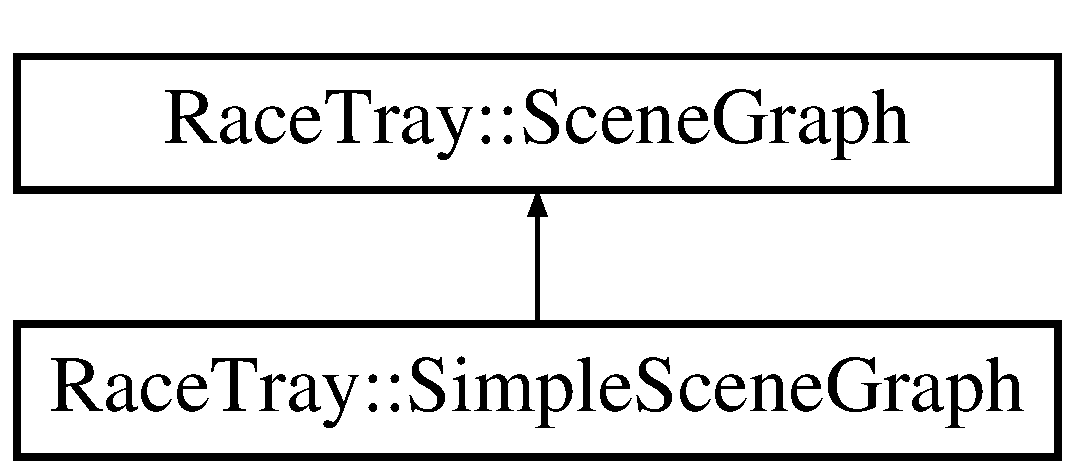
\includegraphics[height=2.000000cm]{class_race_tray_1_1_scene_graph}
\end{center}
\end{figure}
\subsection*{Public Member Functions}
\begin{DoxyCompactItemize}
\item 
\hyperlink{class_race_tray_1_1_scene_graph_a515e791e169aedb48a8ce7d1ccf2ee98}{Scene\-Graph} ()
\item 
\hyperlink{class_race_tray_1_1_scene_graph_ae773263e5bf2b68eacb517c679e9e0c4}{$\sim$\-Scene\-Graph} ()
\item 
virtual bool \hyperlink{class_race_tray_1_1_scene_graph_ac6fcc253f175397971d742747b1bbc6f}{initialize} ()=0
\item 
virtual void \hyperlink{class_race_tray_1_1_scene_graph_a856688d0b5182658c8e9d62bfbc54d6c}{add} (\hyperlink{class_race_tray_1_1_object}{Object} $\ast$object)=0
\end{DoxyCompactItemize}


\subsection{Detailed Description}
The scene graph contains all physical scene information, including objects, particles, etc. 

\subsection{Constructor \& Destructor Documentation}
\hypertarget{class_race_tray_1_1_scene_graph_a515e791e169aedb48a8ce7d1ccf2ee98}{\index{Race\-Tray\-::\-Scene\-Graph@{Race\-Tray\-::\-Scene\-Graph}!Scene\-Graph@{Scene\-Graph}}
\index{Scene\-Graph@{Scene\-Graph}!RaceTray::SceneGraph@{Race\-Tray\-::\-Scene\-Graph}}
\subsubsection[{Scene\-Graph}]{\setlength{\rightskip}{0pt plus 5cm}Race\-Tray\-::\-Scene\-Graph\-::\-Scene\-Graph (
\begin{DoxyParamCaption}
{}
\end{DoxyParamCaption}
)}}\label{class_race_tray_1_1_scene_graph_a515e791e169aedb48a8ce7d1ccf2ee98}
Default constructor \hypertarget{class_race_tray_1_1_scene_graph_ae773263e5bf2b68eacb517c679e9e0c4}{\index{Race\-Tray\-::\-Scene\-Graph@{Race\-Tray\-::\-Scene\-Graph}!$\sim$\-Scene\-Graph@{$\sim$\-Scene\-Graph}}
\index{$\sim$\-Scene\-Graph@{$\sim$\-Scene\-Graph}!RaceTray::SceneGraph@{Race\-Tray\-::\-Scene\-Graph}}
\subsubsection[{$\sim$\-Scene\-Graph}]{\setlength{\rightskip}{0pt plus 5cm}Race\-Tray\-::\-Scene\-Graph\-::$\sim$\-Scene\-Graph (
\begin{DoxyParamCaption}
{}
\end{DoxyParamCaption}
)}}\label{class_race_tray_1_1_scene_graph_ae773263e5bf2b68eacb517c679e9e0c4}
Destructor 

\subsection{Member Function Documentation}
\hypertarget{class_race_tray_1_1_scene_graph_a856688d0b5182658c8e9d62bfbc54d6c}{\index{Race\-Tray\-::\-Scene\-Graph@{Race\-Tray\-::\-Scene\-Graph}!add@{add}}
\index{add@{add}!RaceTray::SceneGraph@{Race\-Tray\-::\-Scene\-Graph}}
\subsubsection[{add}]{\setlength{\rightskip}{0pt plus 5cm}virtual void Race\-Tray\-::\-Scene\-Graph\-::add (
\begin{DoxyParamCaption}
\item[{{\bf Object} $\ast$}]{object}
\end{DoxyParamCaption}
)\hspace{0.3cm}{\ttfamily [pure virtual]}}}\label{class_race_tray_1_1_scene_graph_a856688d0b5182658c8e9d62bfbc54d6c}
Add an object to the scene graph 
\begin{DoxyParams}{Parameters}
{\em Object$\ast$} & The object being added \\
\hline
\end{DoxyParams}


Implemented in \hyperlink{class_race_tray_1_1_simple_scene_graph_a5e10feecf7d0ddaa420bcdee20a4e4dc}{Race\-Tray\-::\-Simple\-Scene\-Graph}.

\hypertarget{class_race_tray_1_1_scene_graph_ac6fcc253f175397971d742747b1bbc6f}{\index{Race\-Tray\-::\-Scene\-Graph@{Race\-Tray\-::\-Scene\-Graph}!initialize@{initialize}}
\index{initialize@{initialize}!RaceTray::SceneGraph@{Race\-Tray\-::\-Scene\-Graph}}
\subsubsection[{initialize}]{\setlength{\rightskip}{0pt plus 5cm}virtual bool Race\-Tray\-::\-Scene\-Graph\-::initialize (
\begin{DoxyParamCaption}
{}
\end{DoxyParamCaption}
)\hspace{0.3cm}{\ttfamily [pure virtual]}}}\label{class_race_tray_1_1_scene_graph_ac6fcc253f175397971d742747b1bbc6f}
Initialize the scene graph \begin{DoxyReturn}{Returns}
bool Returns true if successful 
\end{DoxyReturn}


Implemented in \hyperlink{class_race_tray_1_1_simple_scene_graph_a0e8c2a6b8224a7fa473f729a781c372a}{Race\-Tray\-::\-Simple\-Scene\-Graph}.



The documentation for this class was generated from the following files\-:\begin{DoxyCompactItemize}
\item 
C\-:/\-Users/\-Gael/\-Documents/\-Race\-Tray/\-Scene/R\-T\-Scene\-Graph.\-h\item 
C\-:/\-Users/\-Gael/\-Documents/\-Race\-Tray/\-Scene/R\-T\-Scene\-Graph.\-cpp\end{DoxyCompactItemize}

\hypertarget{class_race_tray_1_1_simple_scene_builder}{\section{Race\-Tray\-:\-:Simple\-Scene\-Builder Class Reference}
\label{class_race_tray_1_1_simple_scene_builder}\index{Race\-Tray\-::\-Simple\-Scene\-Builder@{Race\-Tray\-::\-Simple\-Scene\-Builder}}
}


{\ttfamily \#include $<$R\-T\-Simple\-Scene\-Builder.\-h$>$}

Inheritance diagram for Race\-Tray\-:\-:Simple\-Scene\-Builder\-:\begin{figure}[H]
\begin{center}
\leavevmode
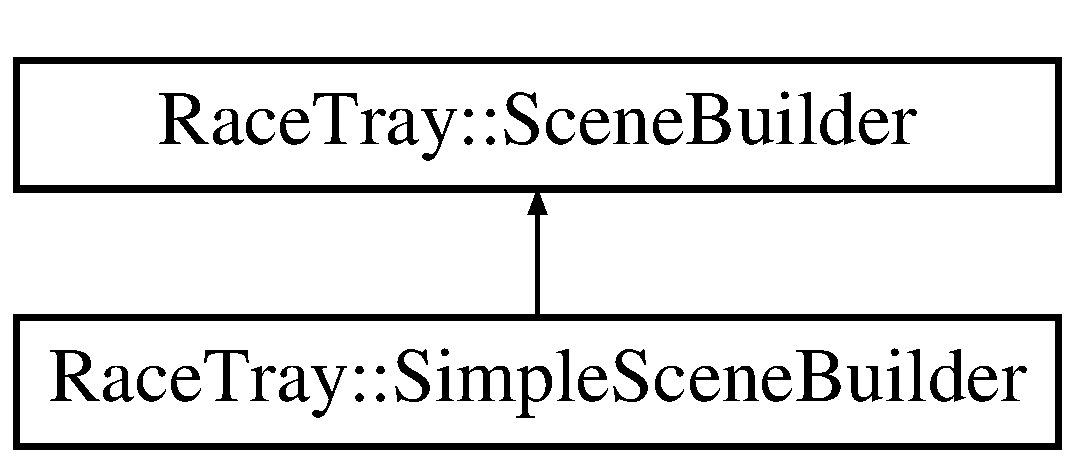
\includegraphics[height=2.000000cm]{class_race_tray_1_1_simple_scene_builder}
\end{center}
\end{figure}
\subsection*{Public Member Functions}
\begin{DoxyCompactItemize}
\item 
\hyperlink{class_race_tray_1_1_simple_scene_builder_adabab20037611d8b93ee191367cff057}{Simple\-Scene\-Builder} ()
\item 
\hyperlink{class_race_tray_1_1_simple_scene_builder_a68f882dca0608b23e6b8fdad7dc22777}{$\sim$\-Simple\-Scene\-Builder} ()
\item 
bool \hyperlink{class_race_tray_1_1_simple_scene_builder_ae4a08c2dae004e17f95a30cbf8249c8b}{build\-Scene} (\hyperlink{class_race_tray_1_1_scene}{Scene} $\ast$scene)
\end{DoxyCompactItemize}


\subsection{Detailed Description}
A simple scene builder constructs a random scene with primitive shapes. 

\subsection{Constructor \& Destructor Documentation}
\hypertarget{class_race_tray_1_1_simple_scene_builder_adabab20037611d8b93ee191367cff057}{\index{Race\-Tray\-::\-Simple\-Scene\-Builder@{Race\-Tray\-::\-Simple\-Scene\-Builder}!Simple\-Scene\-Builder@{Simple\-Scene\-Builder}}
\index{Simple\-Scene\-Builder@{Simple\-Scene\-Builder}!RaceTray::SimpleSceneBuilder@{Race\-Tray\-::\-Simple\-Scene\-Builder}}
\subsubsection[{Simple\-Scene\-Builder}]{\setlength{\rightskip}{0pt plus 5cm}Race\-Tray\-::\-Simple\-Scene\-Builder\-::\-Simple\-Scene\-Builder (
\begin{DoxyParamCaption}
{}
\end{DoxyParamCaption}
)}}\label{class_race_tray_1_1_simple_scene_builder_adabab20037611d8b93ee191367cff057}
Default constructor \hypertarget{class_race_tray_1_1_simple_scene_builder_a68f882dca0608b23e6b8fdad7dc22777}{\index{Race\-Tray\-::\-Simple\-Scene\-Builder@{Race\-Tray\-::\-Simple\-Scene\-Builder}!$\sim$\-Simple\-Scene\-Builder@{$\sim$\-Simple\-Scene\-Builder}}
\index{$\sim$\-Simple\-Scene\-Builder@{$\sim$\-Simple\-Scene\-Builder}!RaceTray::SimpleSceneBuilder@{Race\-Tray\-::\-Simple\-Scene\-Builder}}
\subsubsection[{$\sim$\-Simple\-Scene\-Builder}]{\setlength{\rightskip}{0pt plus 5cm}Race\-Tray\-::\-Simple\-Scene\-Builder\-::$\sim$\-Simple\-Scene\-Builder (
\begin{DoxyParamCaption}
{}
\end{DoxyParamCaption}
)}}\label{class_race_tray_1_1_simple_scene_builder_a68f882dca0608b23e6b8fdad7dc22777}
Destructor 

\subsection{Member Function Documentation}
\hypertarget{class_race_tray_1_1_simple_scene_builder_ae4a08c2dae004e17f95a30cbf8249c8b}{\index{Race\-Tray\-::\-Simple\-Scene\-Builder@{Race\-Tray\-::\-Simple\-Scene\-Builder}!build\-Scene@{build\-Scene}}
\index{build\-Scene@{build\-Scene}!RaceTray::SimpleSceneBuilder@{Race\-Tray\-::\-Simple\-Scene\-Builder}}
\subsubsection[{build\-Scene}]{\setlength{\rightskip}{0pt plus 5cm}bool Race\-Tray\-::\-Simple\-Scene\-Builder\-::build\-Scene (
\begin{DoxyParamCaption}
\item[{{\bf Scene} $\ast$}]{scene}
\end{DoxyParamCaption}
)\hspace{0.3cm}{\ttfamily [virtual]}}}\label{class_race_tray_1_1_simple_scene_builder_ae4a08c2dae004e17f95a30cbf8249c8b}
Build the scene 
\begin{DoxyParams}{Parameters}
{\em Scene$\ast$} & The scene to build \\
\hline
\end{DoxyParams}


Implements \hyperlink{class_race_tray_1_1_scene_builder_abc2dfdc80fe63a47292e5d6f4618d26f}{Race\-Tray\-::\-Scene\-Builder}.



The documentation for this class was generated from the following files\-:\begin{DoxyCompactItemize}
\item 
C\-:/\-Users/\-Gael/\-Documents/\-Race\-Tray/\-Scene/R\-T\-Simple\-Scene\-Builder.\-h\item 
C\-:/\-Users/\-Gael/\-Documents/\-Race\-Tray/\-Scene/R\-T\-Simple\-Scene\-Builder.\-cpp\end{DoxyCompactItemize}

\hypertarget{class_race_tray_1_1_simple_scene_graph}{\section{Race\-Tray\-:\-:Simple\-Scene\-Graph Class Reference}
\label{class_race_tray_1_1_simple_scene_graph}\index{Race\-Tray\-::\-Simple\-Scene\-Graph@{Race\-Tray\-::\-Simple\-Scene\-Graph}}
}


{\ttfamily \#include $<$R\-T\-Simple\-Scene\-Graph.\-h$>$}

Inheritance diagram for Race\-Tray\-:\-:Simple\-Scene\-Graph\-:\begin{figure}[H]
\begin{center}
\leavevmode
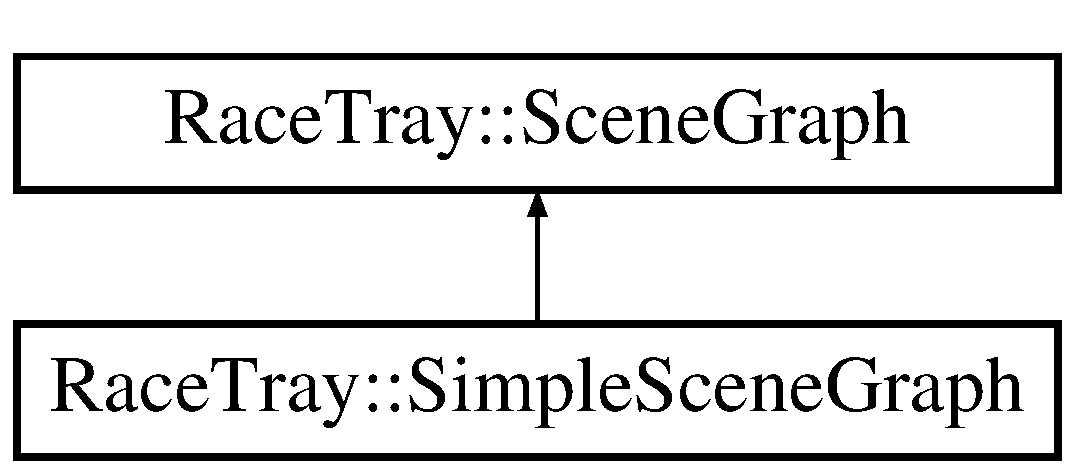
\includegraphics[height=2.000000cm]{class_race_tray_1_1_simple_scene_graph}
\end{center}
\end{figure}
\subsection*{Public Member Functions}
\begin{DoxyCompactItemize}
\item 
\hyperlink{class_race_tray_1_1_simple_scene_graph_a52781b41db73fe219fd5028811292dcb}{Simple\-Scene\-Graph} ()
\item 
\hyperlink{class_race_tray_1_1_simple_scene_graph_a80dbbdc5a7736f2b527ffe1b59d77c85}{$\sim$\-Simple\-Scene\-Graph} ()
\item 
bool \hyperlink{class_race_tray_1_1_simple_scene_graph_a0e8c2a6b8224a7fa473f729a781c372a}{initialize} ()
\item 
void \hyperlink{class_race_tray_1_1_simple_scene_graph_a5e10feecf7d0ddaa420bcdee20a4e4dc}{add} (\hyperlink{class_race_tray_1_1_object}{Object} $\ast$object)
\end{DoxyCompactItemize}


\subsection{Detailed Description}
The scene graph contains all physical scene information, including objects, particles, etc. A simple scene graph uses std\-::vectors and naive search methods for querying the scene. 

\subsection{Constructor \& Destructor Documentation}
\hypertarget{class_race_tray_1_1_simple_scene_graph_a52781b41db73fe219fd5028811292dcb}{\index{Race\-Tray\-::\-Simple\-Scene\-Graph@{Race\-Tray\-::\-Simple\-Scene\-Graph}!Simple\-Scene\-Graph@{Simple\-Scene\-Graph}}
\index{Simple\-Scene\-Graph@{Simple\-Scene\-Graph}!RaceTray::SimpleSceneGraph@{Race\-Tray\-::\-Simple\-Scene\-Graph}}
\subsubsection[{Simple\-Scene\-Graph}]{\setlength{\rightskip}{0pt plus 5cm}Race\-Tray\-::\-Simple\-Scene\-Graph\-::\-Simple\-Scene\-Graph (
\begin{DoxyParamCaption}
{}
\end{DoxyParamCaption}
)}}\label{class_race_tray_1_1_simple_scene_graph_a52781b41db73fe219fd5028811292dcb}
Constructor \hypertarget{class_race_tray_1_1_simple_scene_graph_a80dbbdc5a7736f2b527ffe1b59d77c85}{\index{Race\-Tray\-::\-Simple\-Scene\-Graph@{Race\-Tray\-::\-Simple\-Scene\-Graph}!$\sim$\-Simple\-Scene\-Graph@{$\sim$\-Simple\-Scene\-Graph}}
\index{$\sim$\-Simple\-Scene\-Graph@{$\sim$\-Simple\-Scene\-Graph}!RaceTray::SimpleSceneGraph@{Race\-Tray\-::\-Simple\-Scene\-Graph}}
\subsubsection[{$\sim$\-Simple\-Scene\-Graph}]{\setlength{\rightskip}{0pt plus 5cm}Race\-Tray\-::\-Simple\-Scene\-Graph\-::$\sim$\-Simple\-Scene\-Graph (
\begin{DoxyParamCaption}
{}
\end{DoxyParamCaption}
)}}\label{class_race_tray_1_1_simple_scene_graph_a80dbbdc5a7736f2b527ffe1b59d77c85}
Destructor 

\subsection{Member Function Documentation}
\hypertarget{class_race_tray_1_1_simple_scene_graph_a5e10feecf7d0ddaa420bcdee20a4e4dc}{\index{Race\-Tray\-::\-Simple\-Scene\-Graph@{Race\-Tray\-::\-Simple\-Scene\-Graph}!add@{add}}
\index{add@{add}!RaceTray::SimpleSceneGraph@{Race\-Tray\-::\-Simple\-Scene\-Graph}}
\subsubsection[{add}]{\setlength{\rightskip}{0pt plus 5cm}void Race\-Tray\-::\-Simple\-Scene\-Graph\-::add (
\begin{DoxyParamCaption}
\item[{{\bf Object} $\ast$}]{object}
\end{DoxyParamCaption}
)\hspace{0.3cm}{\ttfamily [virtual]}}}\label{class_race_tray_1_1_simple_scene_graph_a5e10feecf7d0ddaa420bcdee20a4e4dc}
Add an object to the scene graph 
\begin{DoxyParams}{Parameters}
{\em Object$\ast$} & The object being added \\
\hline
\end{DoxyParams}


Implements \hyperlink{class_race_tray_1_1_scene_graph_a856688d0b5182658c8e9d62bfbc54d6c}{Race\-Tray\-::\-Scene\-Graph}.

\hypertarget{class_race_tray_1_1_simple_scene_graph_a0e8c2a6b8224a7fa473f729a781c372a}{\index{Race\-Tray\-::\-Simple\-Scene\-Graph@{Race\-Tray\-::\-Simple\-Scene\-Graph}!initialize@{initialize}}
\index{initialize@{initialize}!RaceTray::SimpleSceneGraph@{Race\-Tray\-::\-Simple\-Scene\-Graph}}
\subsubsection[{initialize}]{\setlength{\rightskip}{0pt plus 5cm}bool Race\-Tray\-::\-Simple\-Scene\-Graph\-::initialize (
\begin{DoxyParamCaption}
{}
\end{DoxyParamCaption}
)\hspace{0.3cm}{\ttfamily [virtual]}}}\label{class_race_tray_1_1_simple_scene_graph_a0e8c2a6b8224a7fa473f729a781c372a}
Initialize the scene graph \begin{DoxyReturn}{Returns}
bool Returns true if successful 
\end{DoxyReturn}


Implements \hyperlink{class_race_tray_1_1_scene_graph_ac6fcc253f175397971d742747b1bbc6f}{Race\-Tray\-::\-Scene\-Graph}.



The documentation for this class was generated from the following files\-:\begin{DoxyCompactItemize}
\item 
C\-:/\-Users/\-Gael/\-Documents/\-Race\-Tray/\-Scene/R\-T\-Simple\-Scene\-Graph.\-h\item 
C\-:/\-Users/\-Gael/\-Documents/\-Race\-Tray/\-Scene/R\-T\-Simple\-Scene\-Graph.\-cpp\end{DoxyCompactItemize}

\hypertarget{class_race_tray_1_1_sphere}{\section{Race\-Tray\-:\-:Sphere Class Reference}
\label{class_race_tray_1_1_sphere}\index{Race\-Tray\-::\-Sphere@{Race\-Tray\-::\-Sphere}}
}


{\ttfamily \#include $<$R\-T\-Sphere.\-h$>$}

Inheritance diagram for Race\-Tray\-:\-:Sphere\-:\begin{figure}[H]
\begin{center}
\leavevmode
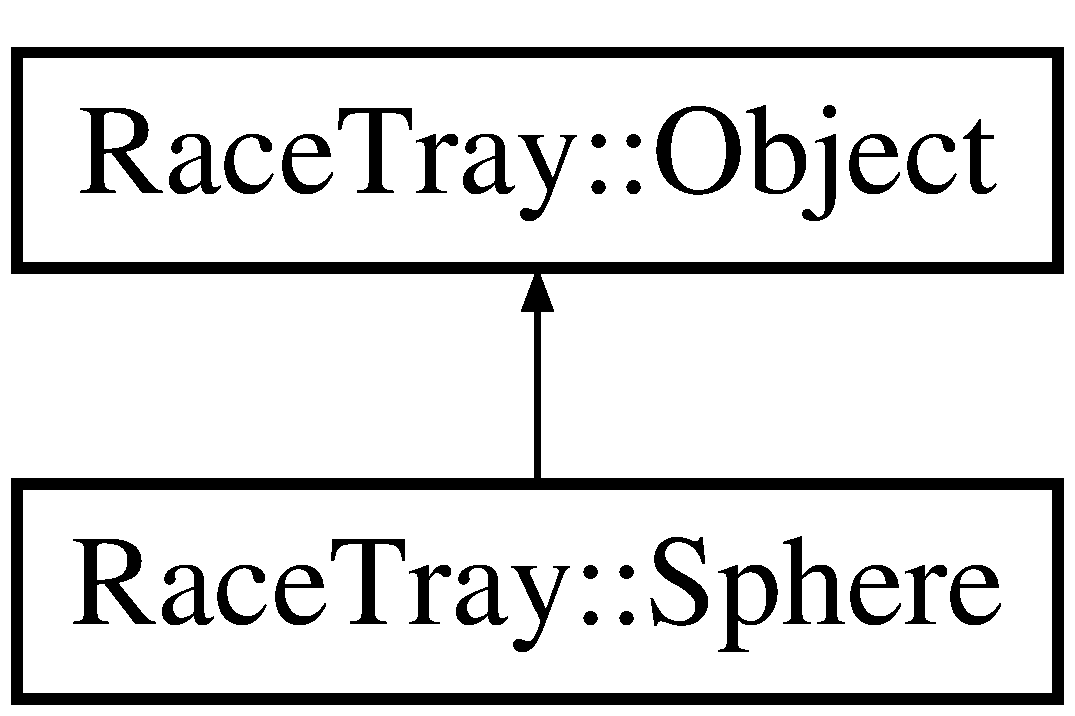
\includegraphics[height=2.000000cm]{class_race_tray_1_1_sphere}
\end{center}
\end{figure}
\subsection*{Public Member Functions}
\begin{DoxyCompactItemize}
\item 
\hyperlink{class_race_tray_1_1_sphere_ab4eadefc469c162c0dfc943d90a88279}{Sphere} ()
\item 
\hyperlink{class_race_tray_1_1_sphere_a80375db61b09ba29ee6dacae567e28b8}{Sphere} (const \hyperlink{group___math_gadb6fa781064c3c3c9b13eb984adae162}{Vector3f} \&position, float radius)
\item 
\hyperlink{class_race_tray_1_1_sphere_a29714dd1da1688b1e150f2f32d6ce05a}{Sphere} (const \hyperlink{class_race_tray_1_1_sphere}{Sphere} \&other)
\item 
\hyperlink{class_race_tray_1_1_sphere_a6b6f93c73945477e091934e26cbe46f2}{$\sim$\-Sphere} ()
\item 
void \hyperlink{class_race_tray_1_1_sphere_a88cf632d6caf1ec6a0ce46efafd6f052}{check\-Ray\-Collision} (const \hyperlink{group___math_ga5fdea6c2a8db84c0cc5b7aaeeb48b17a}{Rayf} \&ray, \hyperlink{class_race_tray_1_1_scene_collision_data}{Scene\-Collision\-Data} \&data)
\end{DoxyCompactItemize}
\subsection*{Additional Inherited Members}


\subsection{Detailed Description}
The base object. All engine entities derive from the base object. 

\subsection{Constructor \& Destructor Documentation}
\hypertarget{class_race_tray_1_1_sphere_ab4eadefc469c162c0dfc943d90a88279}{\index{Race\-Tray\-::\-Sphere@{Race\-Tray\-::\-Sphere}!Sphere@{Sphere}}
\index{Sphere@{Sphere}!RaceTray::Sphere@{Race\-Tray\-::\-Sphere}}
\subsubsection[{Sphere}]{\setlength{\rightskip}{0pt plus 5cm}Race\-Tray\-::\-Sphere\-::\-Sphere (
\begin{DoxyParamCaption}
{}
\end{DoxyParamCaption}
)}}\label{class_race_tray_1_1_sphere_ab4eadefc469c162c0dfc943d90a88279}
Default constructor. The default radius for a sphere is 1m \hypertarget{class_race_tray_1_1_sphere_a80375db61b09ba29ee6dacae567e28b8}{\index{Race\-Tray\-::\-Sphere@{Race\-Tray\-::\-Sphere}!Sphere@{Sphere}}
\index{Sphere@{Sphere}!RaceTray::Sphere@{Race\-Tray\-::\-Sphere}}
\subsubsection[{Sphere}]{\setlength{\rightskip}{0pt plus 5cm}Race\-Tray\-::\-Sphere\-::\-Sphere (
\begin{DoxyParamCaption}
\item[{const {\bf Vector3f} \&}]{position, }
\item[{float}]{radius}
\end{DoxyParamCaption}
)}}\label{class_race_tray_1_1_sphere_a80375db61b09ba29ee6dacae567e28b8}
Constructor 
\begin{DoxyParams}{Parameters}
{\em const} & Vector3f The sphere's position \\
\hline
{\em float} & The radius of the sphere \\
\hline
\end{DoxyParams}
\hypertarget{class_race_tray_1_1_sphere_a29714dd1da1688b1e150f2f32d6ce05a}{\index{Race\-Tray\-::\-Sphere@{Race\-Tray\-::\-Sphere}!Sphere@{Sphere}}
\index{Sphere@{Sphere}!RaceTray::Sphere@{Race\-Tray\-::\-Sphere}}
\subsubsection[{Sphere}]{\setlength{\rightskip}{0pt plus 5cm}Race\-Tray\-::\-Sphere\-::\-Sphere (
\begin{DoxyParamCaption}
\item[{const {\bf Sphere} \&}]{other}
\end{DoxyParamCaption}
)}}\label{class_race_tray_1_1_sphere_a29714dd1da1688b1e150f2f32d6ce05a}
Copy constructor const \hyperlink{class_race_tray_1_1_sphere}{Sphere}\& The sphere to copy \hypertarget{class_race_tray_1_1_sphere_a6b6f93c73945477e091934e26cbe46f2}{\index{Race\-Tray\-::\-Sphere@{Race\-Tray\-::\-Sphere}!$\sim$\-Sphere@{$\sim$\-Sphere}}
\index{$\sim$\-Sphere@{$\sim$\-Sphere}!RaceTray::Sphere@{Race\-Tray\-::\-Sphere}}
\subsubsection[{$\sim$\-Sphere}]{\setlength{\rightskip}{0pt plus 5cm}Race\-Tray\-::\-Sphere\-::$\sim$\-Sphere (
\begin{DoxyParamCaption}
{}
\end{DoxyParamCaption}
)}}\label{class_race_tray_1_1_sphere_a6b6f93c73945477e091934e26cbe46f2}
Destructor 

\subsection{Member Function Documentation}
\hypertarget{class_race_tray_1_1_sphere_a88cf632d6caf1ec6a0ce46efafd6f052}{\index{Race\-Tray\-::\-Sphere@{Race\-Tray\-::\-Sphere}!check\-Ray\-Collision@{check\-Ray\-Collision}}
\index{check\-Ray\-Collision@{check\-Ray\-Collision}!RaceTray::Sphere@{Race\-Tray\-::\-Sphere}}
\subsubsection[{check\-Ray\-Collision}]{\setlength{\rightskip}{0pt plus 5cm}void Race\-Tray\-::\-Sphere\-::check\-Ray\-Collision (
\begin{DoxyParamCaption}
\item[{const {\bf Rayf} \&}]{ray, }
\item[{{\bf Scene\-Collision\-Data} \&}]{data}
\end{DoxyParamCaption}
)\hspace{0.3cm}{\ttfamily [virtual]}}}\label{class_race_tray_1_1_sphere_a88cf632d6caf1ec6a0ce46efafd6f052}
Check against this object for a ray collision. 
\begin{DoxyParams}{Parameters}
{\em const} & \hyperlink{class_race_tray_1_1_ray}{Ray}\& The ray against which to check \\
\hline
{\em Scene\-Collision\-Data\&} & The information about the collision, if any \\
\hline
\end{DoxyParams}


Implements \hyperlink{class_race_tray_1_1_object_a6ea71904be1d47e93378e58848b6eb87}{Race\-Tray\-::\-Object}.



The documentation for this class was generated from the following files\-:\begin{DoxyCompactItemize}
\item 
C\-:/\-Users/\-Gael/\-Documents/\-Race\-Tray/\-Geometry/R\-T\-Sphere.\-h\item 
C\-:/\-Users/\-Gael/\-Documents/\-Race\-Tray/\-Geometry/R\-T\-Sphere.\-cpp\end{DoxyCompactItemize}

\hypertarget{class_race_tray_1_1_static_render_target}{\section{Race\-Tray\-:\-:Static\-Render\-Target Class Reference}
\label{class_race_tray_1_1_static_render_target}\index{Race\-Tray\-::\-Static\-Render\-Target@{Race\-Tray\-::\-Static\-Render\-Target}}
}


{\ttfamily \#include $<$R\-T\-Static\-Render\-Target.\-h$>$}

Inheritance diagram for Race\-Tray\-:\-:Static\-Render\-Target\-:\begin{figure}[H]
\begin{center}
\leavevmode
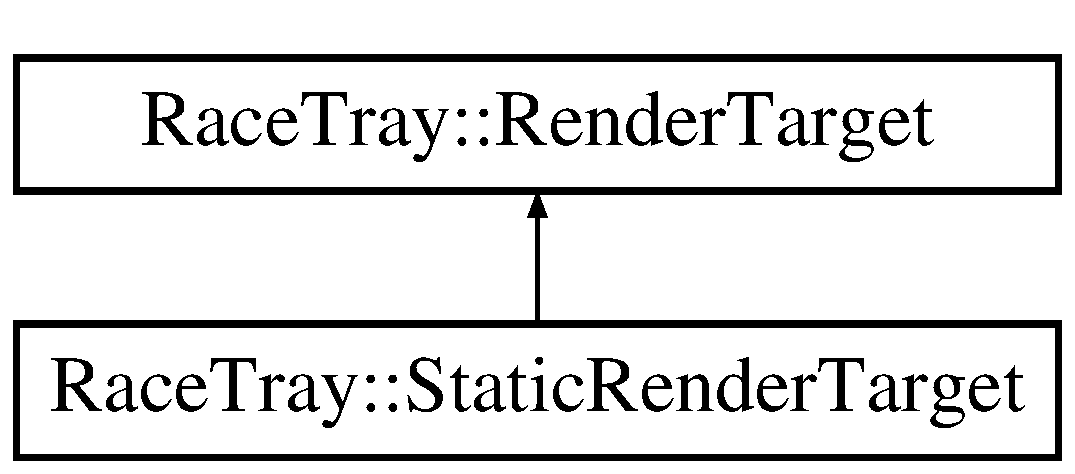
\includegraphics[height=2.000000cm]{class_race_tray_1_1_static_render_target}
\end{center}
\end{figure}
\subsection*{Public Member Functions}
\begin{DoxyCompactItemize}
\item 
\hyperlink{class_race_tray_1_1_static_render_target_aff3df5ac39783e29d0ec62746069d862}{Static\-Render\-Target} ()
\item 
\hyperlink{class_race_tray_1_1_static_render_target_a2443c361f8e5290e88d2380f2993a391}{Static\-Render\-Target} (const \hyperlink{class_race_tray_1_1_static_render_target}{Static\-Render\-Target} \&other)
\item 
\hyperlink{class_race_tray_1_1_static_render_target_a06a1218cf1df44e10dad99b132c2f316}{$\sim$\-Static\-Render\-Target} ()
\item 
bool \hyperlink{class_race_tray_1_1_static_render_target_a4f7bf1080af87d6b64e40771adac1861}{initialize} (int width, int height)
\item 
void \hyperlink{class_race_tray_1_1_static_render_target_a4f163966507ea68a0eccf7c3f5959bd3}{destroy} ()
\end{DoxyCompactItemize}
\subsection*{Additional Inherited Members}


\subsection{Detailed Description}
A static render target contains a simple array buffer to represent screen pixels 

\subsection{Constructor \& Destructor Documentation}
\hypertarget{class_race_tray_1_1_static_render_target_aff3df5ac39783e29d0ec62746069d862}{\index{Race\-Tray\-::\-Static\-Render\-Target@{Race\-Tray\-::\-Static\-Render\-Target}!Static\-Render\-Target@{Static\-Render\-Target}}
\index{Static\-Render\-Target@{Static\-Render\-Target}!RaceTray::StaticRenderTarget@{Race\-Tray\-::\-Static\-Render\-Target}}
\subsubsection[{Static\-Render\-Target}]{\setlength{\rightskip}{0pt plus 5cm}Race\-Tray\-::\-Static\-Render\-Target\-::\-Static\-Render\-Target (
\begin{DoxyParamCaption}
{}
\end{DoxyParamCaption}
)}}\label{class_race_tray_1_1_static_render_target_aff3df5ac39783e29d0ec62746069d862}
Default constructor \hypertarget{class_race_tray_1_1_static_render_target_a2443c361f8e5290e88d2380f2993a391}{\index{Race\-Tray\-::\-Static\-Render\-Target@{Race\-Tray\-::\-Static\-Render\-Target}!Static\-Render\-Target@{Static\-Render\-Target}}
\index{Static\-Render\-Target@{Static\-Render\-Target}!RaceTray::StaticRenderTarget@{Race\-Tray\-::\-Static\-Render\-Target}}
\subsubsection[{Static\-Render\-Target}]{\setlength{\rightskip}{0pt plus 5cm}Race\-Tray\-::\-Static\-Render\-Target\-::\-Static\-Render\-Target (
\begin{DoxyParamCaption}
\item[{const {\bf Static\-Render\-Target} \&}]{other}
\end{DoxyParamCaption}
)}}\label{class_race_tray_1_1_static_render_target_a2443c361f8e5290e88d2380f2993a391}
Copy constructor 
\begin{DoxyParams}{Parameters}
{\em const} & \hyperlink{class_race_tray_1_1_static_render_target}{Static\-Render\-Target}\& The render target to copy \\
\hline
\end{DoxyParams}
\hypertarget{class_race_tray_1_1_static_render_target_a06a1218cf1df44e10dad99b132c2f316}{\index{Race\-Tray\-::\-Static\-Render\-Target@{Race\-Tray\-::\-Static\-Render\-Target}!$\sim$\-Static\-Render\-Target@{$\sim$\-Static\-Render\-Target}}
\index{$\sim$\-Static\-Render\-Target@{$\sim$\-Static\-Render\-Target}!RaceTray::StaticRenderTarget@{Race\-Tray\-::\-Static\-Render\-Target}}
\subsubsection[{$\sim$\-Static\-Render\-Target}]{\setlength{\rightskip}{0pt plus 5cm}Race\-Tray\-::\-Static\-Render\-Target\-::$\sim$\-Static\-Render\-Target (
\begin{DoxyParamCaption}
{}
\end{DoxyParamCaption}
)}}\label{class_race_tray_1_1_static_render_target_a06a1218cf1df44e10dad99b132c2f316}
Destructor 

\subsection{Member Function Documentation}
\hypertarget{class_race_tray_1_1_static_render_target_a4f163966507ea68a0eccf7c3f5959bd3}{\index{Race\-Tray\-::\-Static\-Render\-Target@{Race\-Tray\-::\-Static\-Render\-Target}!destroy@{destroy}}
\index{destroy@{destroy}!RaceTray::StaticRenderTarget@{Race\-Tray\-::\-Static\-Render\-Target}}
\subsubsection[{destroy}]{\setlength{\rightskip}{0pt plus 5cm}void Race\-Tray\-::\-Static\-Render\-Target\-::destroy (
\begin{DoxyParamCaption}
{}
\end{DoxyParamCaption}
)\hspace{0.3cm}{\ttfamily [virtual]}}}\label{class_race_tray_1_1_static_render_target_a4f163966507ea68a0eccf7c3f5959bd3}
Destroy the render target 

Implements \hyperlink{class_race_tray_1_1_render_target_a9e4e394b421102e5edaea14411dc28bd}{Race\-Tray\-::\-Render\-Target}.

\hypertarget{class_race_tray_1_1_static_render_target_a4f7bf1080af87d6b64e40771adac1861}{\index{Race\-Tray\-::\-Static\-Render\-Target@{Race\-Tray\-::\-Static\-Render\-Target}!initialize@{initialize}}
\index{initialize@{initialize}!RaceTray::StaticRenderTarget@{Race\-Tray\-::\-Static\-Render\-Target}}
\subsubsection[{initialize}]{\setlength{\rightskip}{0pt plus 5cm}bool Race\-Tray\-::\-Static\-Render\-Target\-::initialize (
\begin{DoxyParamCaption}
\item[{int}]{width, }
\item[{int}]{height}
\end{DoxyParamCaption}
)\hspace{0.3cm}{\ttfamily [virtual]}}}\label{class_race_tray_1_1_static_render_target_a4f7bf1080af87d6b64e40771adac1861}
Initialize the render target 
\begin{DoxyParams}{Parameters}
{\em int} & The width of the render target \\
\hline
{\em height} & The height of the render target \\
\hline
\end{DoxyParams}
\begin{DoxyReturn}{Returns}
bool Returns true if the target is successfully created 
\end{DoxyReturn}


Implements \hyperlink{class_race_tray_1_1_render_target_a8ac06cc0f9af87e3373cd1514f64b76c}{Race\-Tray\-::\-Render\-Target}.



The documentation for this class was generated from the following files\-:\begin{DoxyCompactItemize}
\item 
C\-:/\-Users/\-Gael/\-Documents/\-Race\-Tray/\-Scene/R\-T\-Static\-Render\-Target.\-h\item 
C\-:/\-Users/\-Gael/\-Documents/\-Race\-Tray/\-Scene/R\-T\-Static\-Render\-Target.\-cpp\end{DoxyCompactItemize}

\hypertarget{class_race_tray_1_1_vector2}{\section{Race\-Tray\-:\-:Vector2$<$ Unit $>$ Class Template Reference}
\label{class_race_tray_1_1_vector2}\index{Race\-Tray\-::\-Vector2$<$ Unit $>$@{Race\-Tray\-::\-Vector2$<$ Unit $>$}}
}


{\ttfamily \#include $<$R\-T\-Vector2.\-h$>$}



\subsection{Detailed Description}
\subsubsection*{template$<$typename Unit$>$class Race\-Tray\-::\-Vector2$<$ Unit $>$}

2-\/dimensional vector mathematics. 

The documentation for this class was generated from the following file\-:\begin{DoxyCompactItemize}
\item 
C\-:/\-Users/\-Gael/\-Documents/\-Race\-Tray/\-Math/R\-T\-Math\-Prerequisites.\-h\end{DoxyCompactItemize}

\hypertarget{class_race_tray_1_1_vector3}{\section{Race\-Tray\-:\-:Vector3$<$ Unit $>$ Class Template Reference}
\label{class_race_tray_1_1_vector3}\index{Race\-Tray\-::\-Vector3$<$ Unit $>$@{Race\-Tray\-::\-Vector3$<$ Unit $>$}}
}


{\ttfamily \#include $<$R\-T\-Vector3.\-h$>$}

\subsection*{Public Member Functions}
\begin{DoxyCompactItemize}
\item 
\hyperlink{group___math_ga0f49191f7e001e7f7ae1cb49522118b4}{Vector3} ()
\item 
\hyperlink{group___math_gaaa5ebab83f6d1f282df85ece8153311d}{Vector3} (Unit x, Unit y, Unit z)
\item 
\hyperlink{group___math_ga1467854ce0d4ef24f84fecf84446910b}{Vector3} (Unit $\ast$coordinates)
\item 
\hyperlink{group___math_ga636420f8171f95d953e80b9752ca98e8}{Vector3} (const \hyperlink{class_race_tray_1_1_vector3}{Vector3} \&value)
\item 
\hyperlink{group___math_ga5545e13e2e2861ece8f14b12a6a8101f}{$\sim$\-Vector3} ()
\item 
\hyperlink{class_race_tray_1_1_vector3}{Vector3} \& \hyperlink{group___math_gadcef1abbe010682b06779beab2fddc9e}{operator=} (const \hyperlink{class_race_tray_1_1_vector3}{Vector3} \&other)
\item 
Unit \hyperlink{group___math_gad352703f15280f9a3e92ab30f8f0a559}{get\-X} () const 
\item 
Unit \hyperlink{group___math_ga958d217bc40bbecc3f7710f7d21d69e2}{get\-Y} () const 
\item 
Unit \hyperlink{group___math_ga78a16de98839cff6799b841cd5dce3a5}{get\-Z} () const 
\item 
Unit \hyperlink{group___math_gac176f26759f013157ae339e037abcbbd}{operator\mbox{[}$\,$\mbox{]}} (int index) const 
\item 
Unit \hyperlink{group___math_ga6a55bfca19953a2b43b30796e4ce3f67}{dot} (const \hyperlink{class_race_tray_1_1_vector3}{Vector3} \&other) const 
\item 
\hyperlink{class_race_tray_1_1_vector3}{Vector3} \hyperlink{group___math_ga3bad6b5bd57c5e674c6cb47e6eb75246}{cross} (const \hyperlink{class_race_tray_1_1_vector3}{Vector3} \&other) const 
\item 
\hyperlink{class_race_tray_1_1_vector3}{Vector3} \hyperlink{group___math_gaf130562c28e9acf79a1947eae9bc583b}{add} (const \hyperlink{class_race_tray_1_1_vector3}{Vector3} \&other) const 
\item 
\hyperlink{class_race_tray_1_1_vector3}{Vector3} \hyperlink{group___math_ga66fc04cc87dd36820cc8cad9d3ba7fae}{operator+} (const \hyperlink{class_race_tray_1_1_vector3}{Vector3} \&other) const 
\item 
\hyperlink{class_race_tray_1_1_vector3}{Vector3} \& \hyperlink{group___math_ga5ccb50254f27230d20aab11372215fbc}{operator+=} (const \hyperlink{class_race_tray_1_1_vector3}{Vector3} \&other)
\item 
\hyperlink{class_race_tray_1_1_vector3}{Vector3} \hyperlink{group___math_ga76645af9d0562c9964fcd0850a327288}{sub} (const \hyperlink{class_race_tray_1_1_vector3}{Vector3} \&other) const 
\item 
\hyperlink{class_race_tray_1_1_vector3}{Vector3} \hyperlink{group___math_gaa69c327bce74c6fccc67732aa72d51e4}{operator-\/} (const \hyperlink{class_race_tray_1_1_vector3}{Vector3} \&other) const 
\item 
\hyperlink{class_race_tray_1_1_vector3}{Vector3} \& \hyperlink{group___math_gae0287f848b8e46e8e2abbaa1a8940f9d}{operator-\/=} (const \hyperlink{class_race_tray_1_1_vector3}{Vector3} \&other)
\item 
\hyperlink{class_race_tray_1_1_vector3}{Vector3} \hyperlink{group___math_ga9282288d74a882eb1b049abc21f8b0c7}{scale} (Unit scale) const 
\item 
\hyperlink{class_race_tray_1_1_vector3}{Vector3} \hyperlink{group___math_ga89a8462c9f9c3802cbc7092f234e9a04}{operator$\ast$} (Unit \hyperlink{group___math_ga9282288d74a882eb1b049abc21f8b0c7}{scale}) const 
\item 
\hyperlink{class_race_tray_1_1_vector3}{Vector3} \& \hyperlink{group___math_gaf2ead3fae3ec911d2d0ece2c88f0488c}{operator$\ast$=} (Unit \hyperlink{group___math_ga9282288d74a882eb1b049abc21f8b0c7}{scale})
\item 
Unit \hyperlink{group___math_ga060ae22a7ea4202c7d401bbcb0c0732d}{length} () const 
\item 
Unit \hyperlink{group___math_ga0642d7d561ce609f96b1df8ad6c8bb8a}{sqr\-Length} () const 
\item 
\hyperlink{class_race_tray_1_1_vector3}{Vector3} \hyperlink{group___math_ga822111c5601c2d6b8dab069acd2df835}{normal} () const 
\item 
\hyperlink{class_race_tray_1_1_vector3}{Vector3} \& \hyperlink{group___math_ga606bb7deceeda5a9cab17e22e1aed668}{normalize} ()
\item 
bool \hyperlink{group___math_gacc0738d9f3ef7de9deb35b27472e6397}{operator==} (const \hyperlink{class_race_tray_1_1_vector3}{Vector3} \&other)
\item 
bool \hyperlink{group___math_ga618208f396f28328642826f06fcab560}{operator!=} (const \hyperlink{class_race_tray_1_1_vector3}{Vector3} \&other)
\end{DoxyCompactItemize}


\subsection{Detailed Description}
\subsubsection*{template$<$typename Unit$>$class Race\-Tray\-::\-Vector3$<$ Unit $>$}

Represents a 3 dimensional vector 

The documentation for this class was generated from the following files\-:\begin{DoxyCompactItemize}
\item 
C\-:/\-Users/\-Gael/\-Documents/\-Race\-Tray/\-Math/R\-T\-Math\-Prerequisites.\-h\item 
C\-:/\-Users/\-Gael/\-Documents/\-Race\-Tray/\-Math/R\-T\-Vector3.\-h\item 
C\-:/\-Users/\-Gael/\-Documents/\-Race\-Tray/\-Math/R\-T\-Vector3.\-inl\end{DoxyCompactItemize}

%--- End generated contents ---

% Index
\newpage
\phantomsection
\addcontentsline{toc}{chapter}{Index}
\printindex

\end{document}
